\documentclass[a4paper,11pt,openany]{book}
\usepackage[utf8]{inputenc}
\usepackage[left=2.54cm,top=2.54cm,right=2.54cm,bottom=2.54cm]{geometry}
\usepackage[spanish]{babel}
\usepackage{amsmath}
\usepackage{amsfonts}
\usepackage{amssymb}
\usepackage{graphicx}
\usepackage{color}
\usepackage[usenames,dvipsnames]{xcolor}
\usepackage{pifont}
\usepackage{marvosym}
\newtheorem{teo}{Teorema}
\newtheorem{ejemplo}{Ejemplo}
\newtheorem{defi}{Definición}
\newtheorem{coro}{Corolario}
\newtheorem{prueba}{Prueba}
\newtheorem{exmp}{Example}[section]
\newtheorem{ejer}{Ejercicio}[section]
\def\proof{\paragraph{\textsf{Demostración.} }}
\def\endproof{\hfill $\blacksquare$ \\}
\usepackage{multirow, array} % para las tablas
\usepackage{multirow}
\usepackage{tabularx}
\usepackage{float} % para usar [H]
\usepackage{tikz}
\usepackage[all]{xy}
\usepackage{cancel}
\usetikzlibrary{positioning}
\usepackage{enumitem}
\newcommand*{\itembolasazules}[1]{% bolas 3D
\footnotesize\protect\tikz[baseline=-3pt]%
\protect\node[scale=.7, circle, shade, ball
color=green]{\color{white}\Large\bf#1};}
\usepackage{tcolorbox} 
\tcbuselibrary{listingsutf8}
\newtcolorbox[auto counter,number within=section]{example}[2][]
{colback=green!5!white,colframe=green!75!black,fonttitle=\bfseries, title=Ejercicio~\thetcbcounter: #2,#1}
\usepackage{background}
\backgroundsetup{
placement=center,
angle=0,
scale=1.1,
contents= {{
\includegraphics{HojaCuadriculada.png}}}
}
 
 
\begin{document}
\begin{titlepage}
 
\begin{center}
\vspace*{-1in}
\begin{figure}[htb]
\begin{center}

\includegraphics[width=7cm]{ETITC.png}
\end{center}
\end{figure}
 
 
{\sc \huge Escuela Tecnológica Instituto Técnico Central (ETITC)}\\
\vspace*{0.15in}
Facultad de sistemas\\
\vspace*{0.6in}
\begin{Large}
\textbf{Taller 3: Conjuntos en el Plano Complejo} \\
\textbf{Matem{\'a}ticas Especiales}\\
\end{Large}
\vspace*{0.3in}
\begin{large}
{\bf Autores} \\
 
\ 
 
Sergio Alejandro Enrrique Caballero Leon\\ 
Johan Alejandro Sogamoso Camacho \\
David Andrés Valero Vanegas \\
\end{large}
\vspace*{0.3in}
 
\end{center}
 
\begin{center}
{\bf Presentado a:} \\
 
\ 
 
Carlos Romero \\
 
\
 
Bogot{\'a}, 8 de Septiembre de 2022.
\end{center}
 
\end{titlepage}

\newpage

\definecolor{ao(english)}{rgb}{0.0, 0.5, 0.0}

\graphicspath{ {images/} }

\begin{center}
\textbf{Conjuntos}
\end{center}

En los ejercicios \textbf{(\,1\,)} al \textbf{(\,12\,) graficar}, cada uno en un plano complejo, el conjunto de puntos $\mathnormal{S}$ que satisface la igualdad o desigualdad dada y \textbf{escribir qué tipo de conjunto es:} Círculo, Disco, Anillo, etc. Además decir si el conjunto es Abierto, Cerrado ó Semi-Abierto (ó Semi-Cerrado).\\

\textcolor{ao(english)}{(\,1\,)} $\bf{|z\,-\,4\,+\,3\,i|\,=\,5}$.

$$|z\,-\,4\,+\,3\,i|\,=\,5 \quad\iff\quad |z\,-\,(4\,-\,3\,i)|\,=\,5$$

el radio del Círculo es $r\,=\,5$ y el centro de este es $z_{0}\,=\,4\,-\,3\,i$.\\

\textcolor{ao(english)}{\ding{47}} Graficar el Círculo.

\begin{center}
     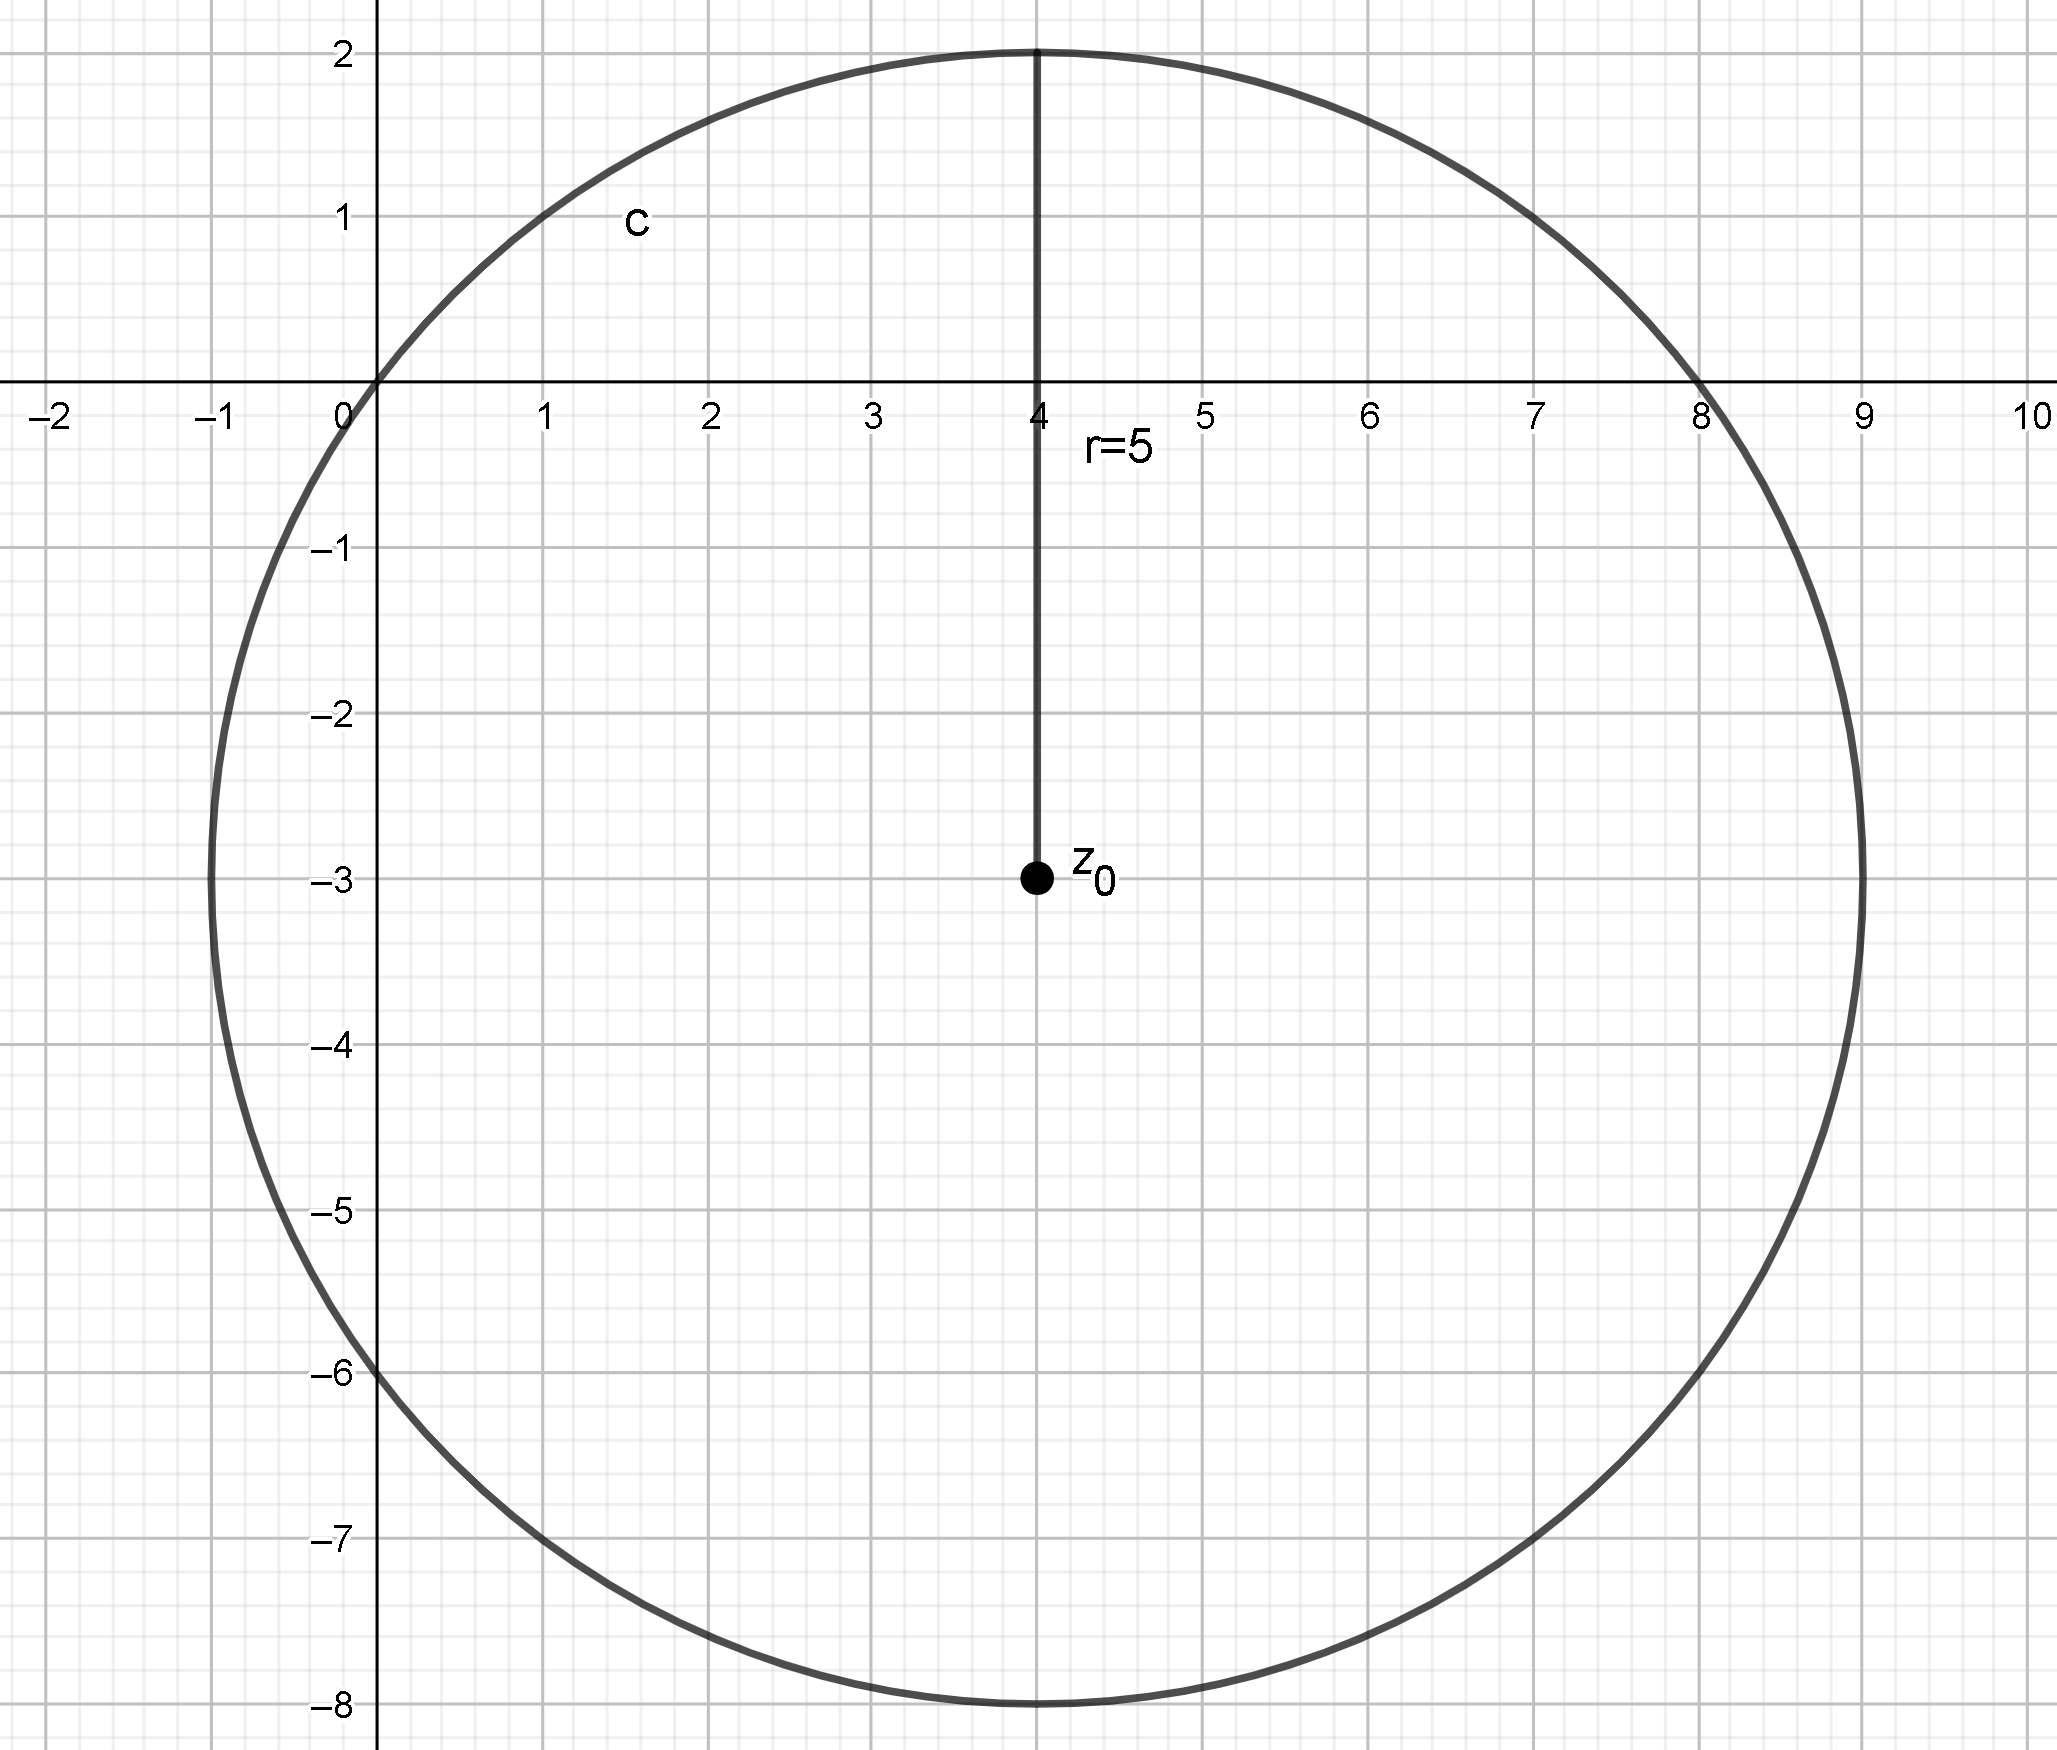
\includegraphics[width=10cm]{Gra-Ej-1.png}
\end{center}

\textcolor{ao(english)}{(\,2\,)} $\bf{|z\,+\,2\,-\,5\,i|\,\leq\,4}$.\\
$\text{Disco cerrado}$

El radio del Círculo es $r\,=\,4$ y el centro de este es $z_{0}\,=-\,2\,+\,5\,i$.\\

\begin{center}
    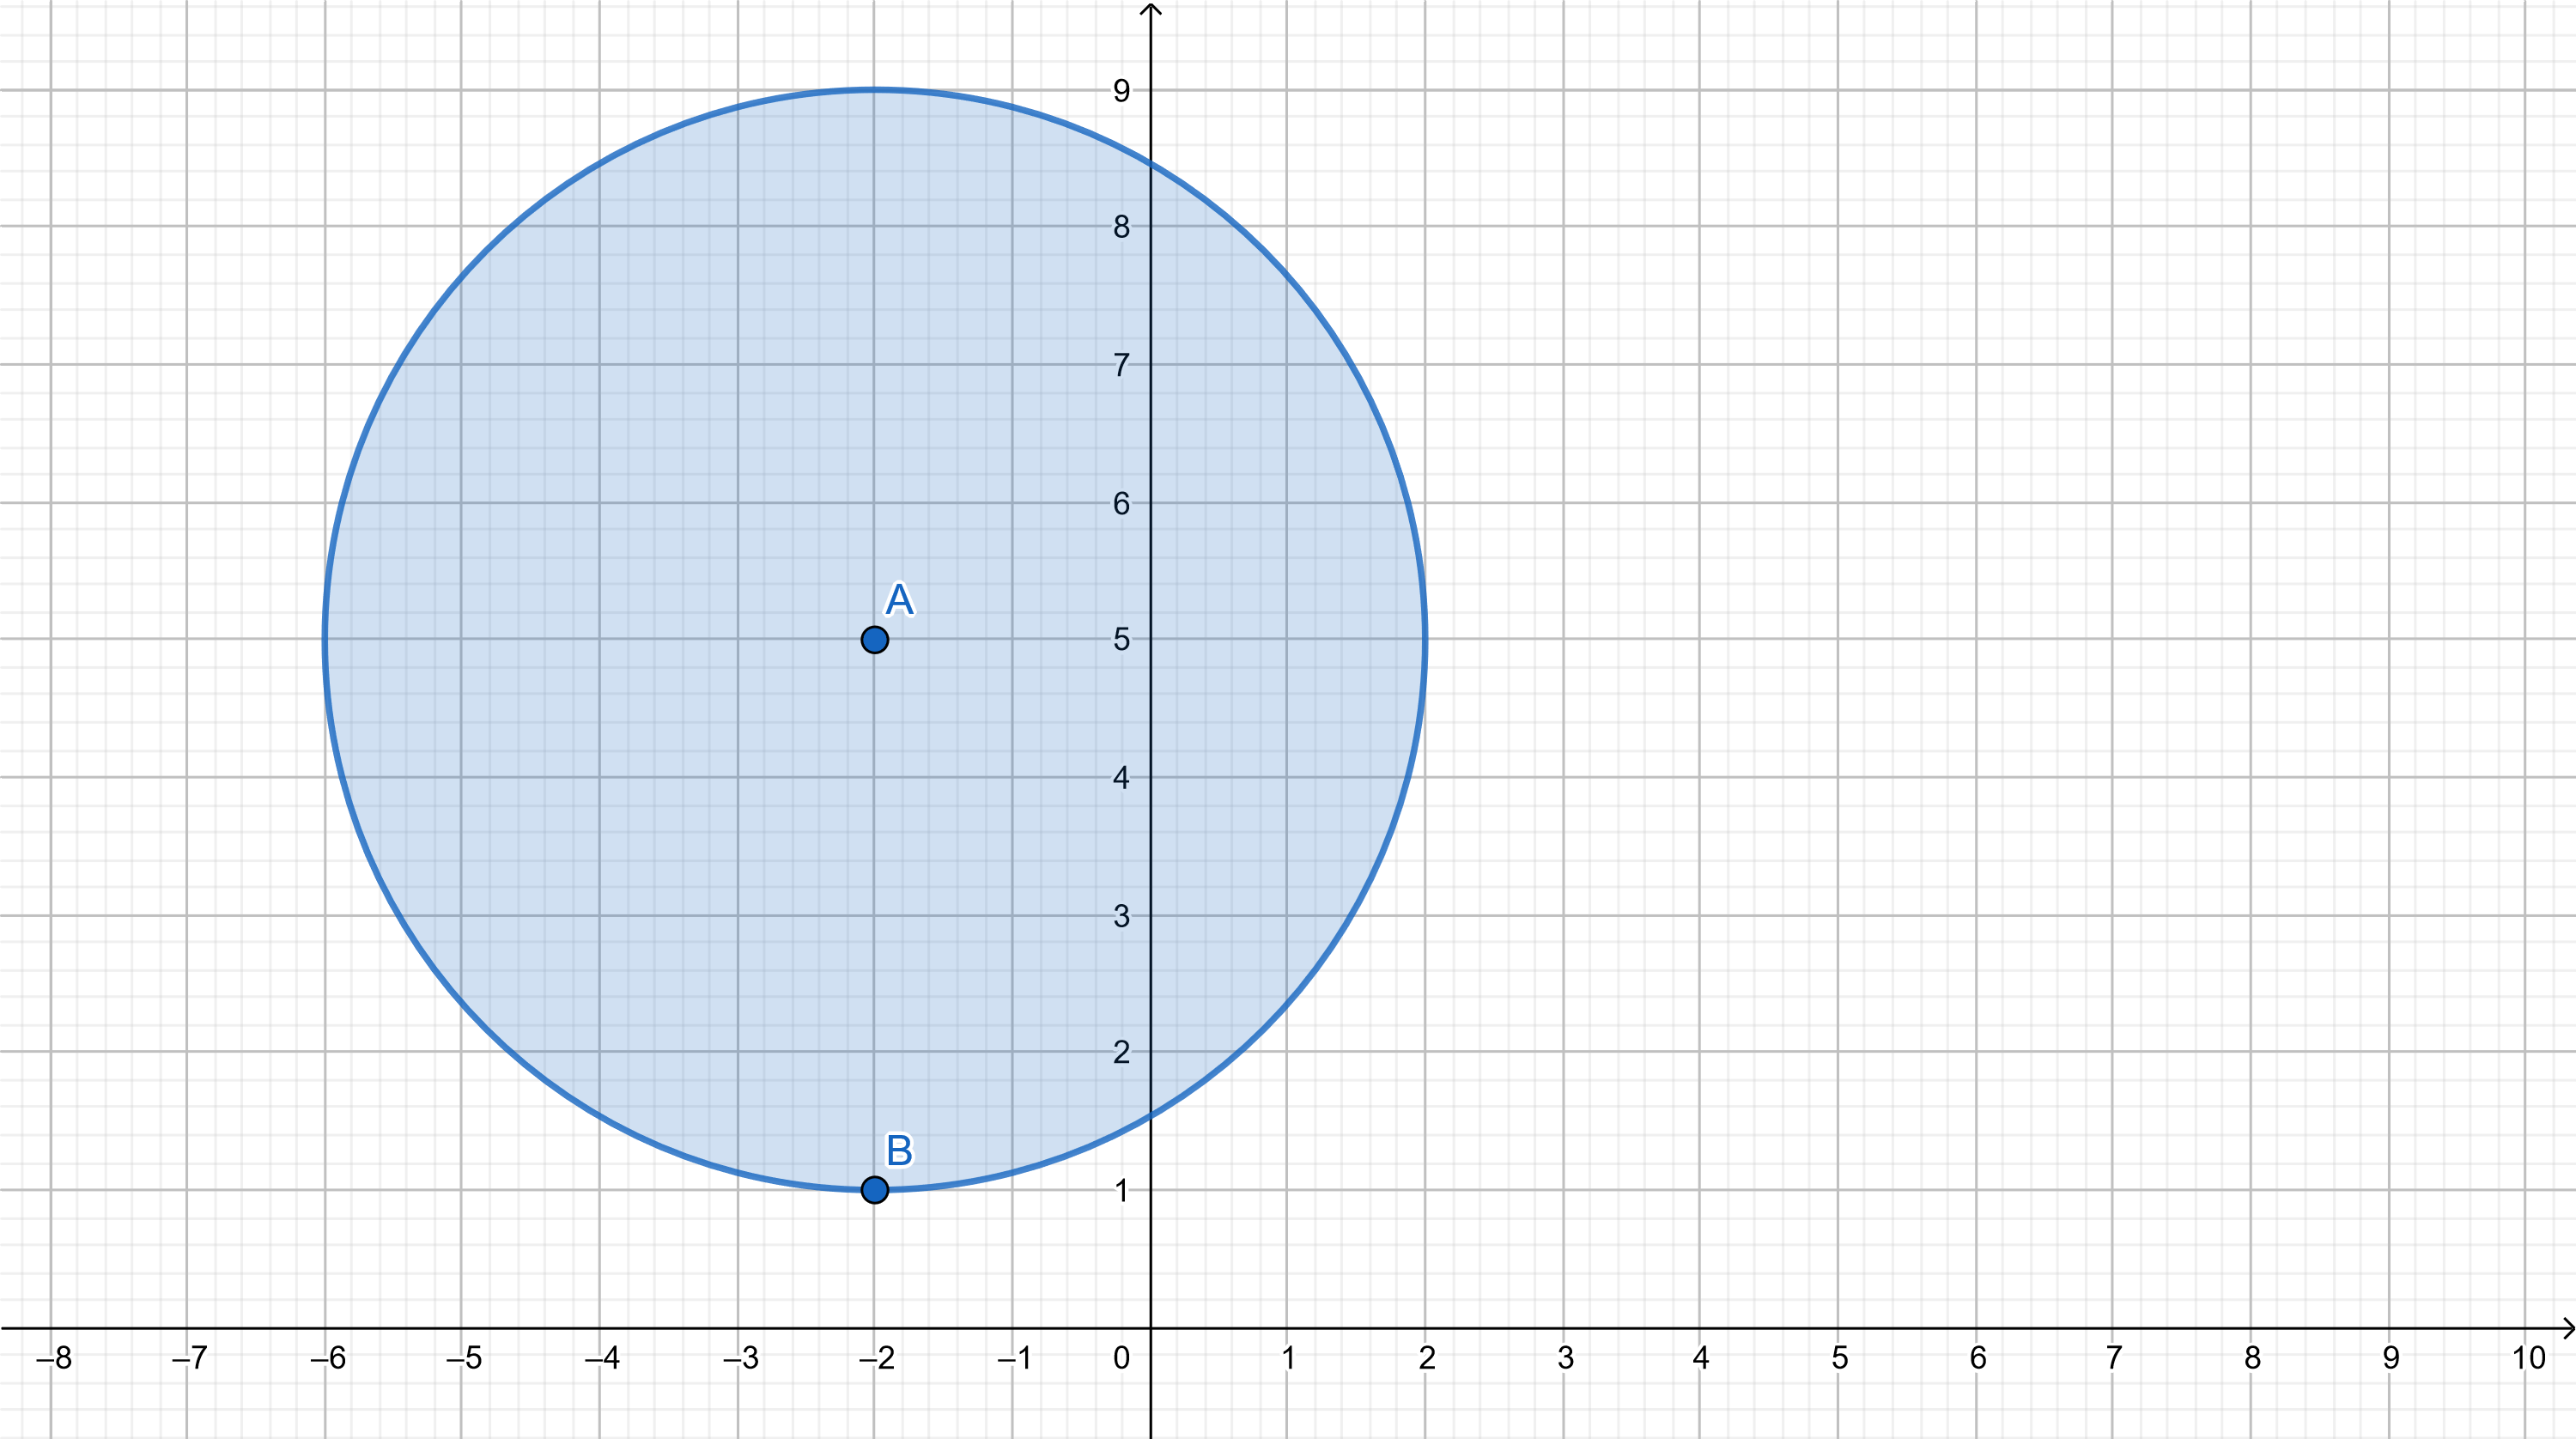
\includegraphics[width=10cm]{Gra-Ej-2.png}
\end{center}

\textcolor{ao(english)}{(\,3\,)} $\bf{2\,\leq\,|z\,+\,3\,i|\,<\,6}$.

$$2\,\leq\,|z\,+\,3\,i|\,<\,6 \quad\iff\quad 2\,\leq\,|z\,-\,(-\,3\,i)|\,<\,6$$

Anillo semiabierto con $\, r_{1}\,=\,2\,,\,r_{2}\,=\,6$ y el centro en $z_{0}\,=\,-\,3\,i$.\\

\textcolor{ao(english)}{\ding{47}} Graficar el anillo semiabierto

\begin{center}
     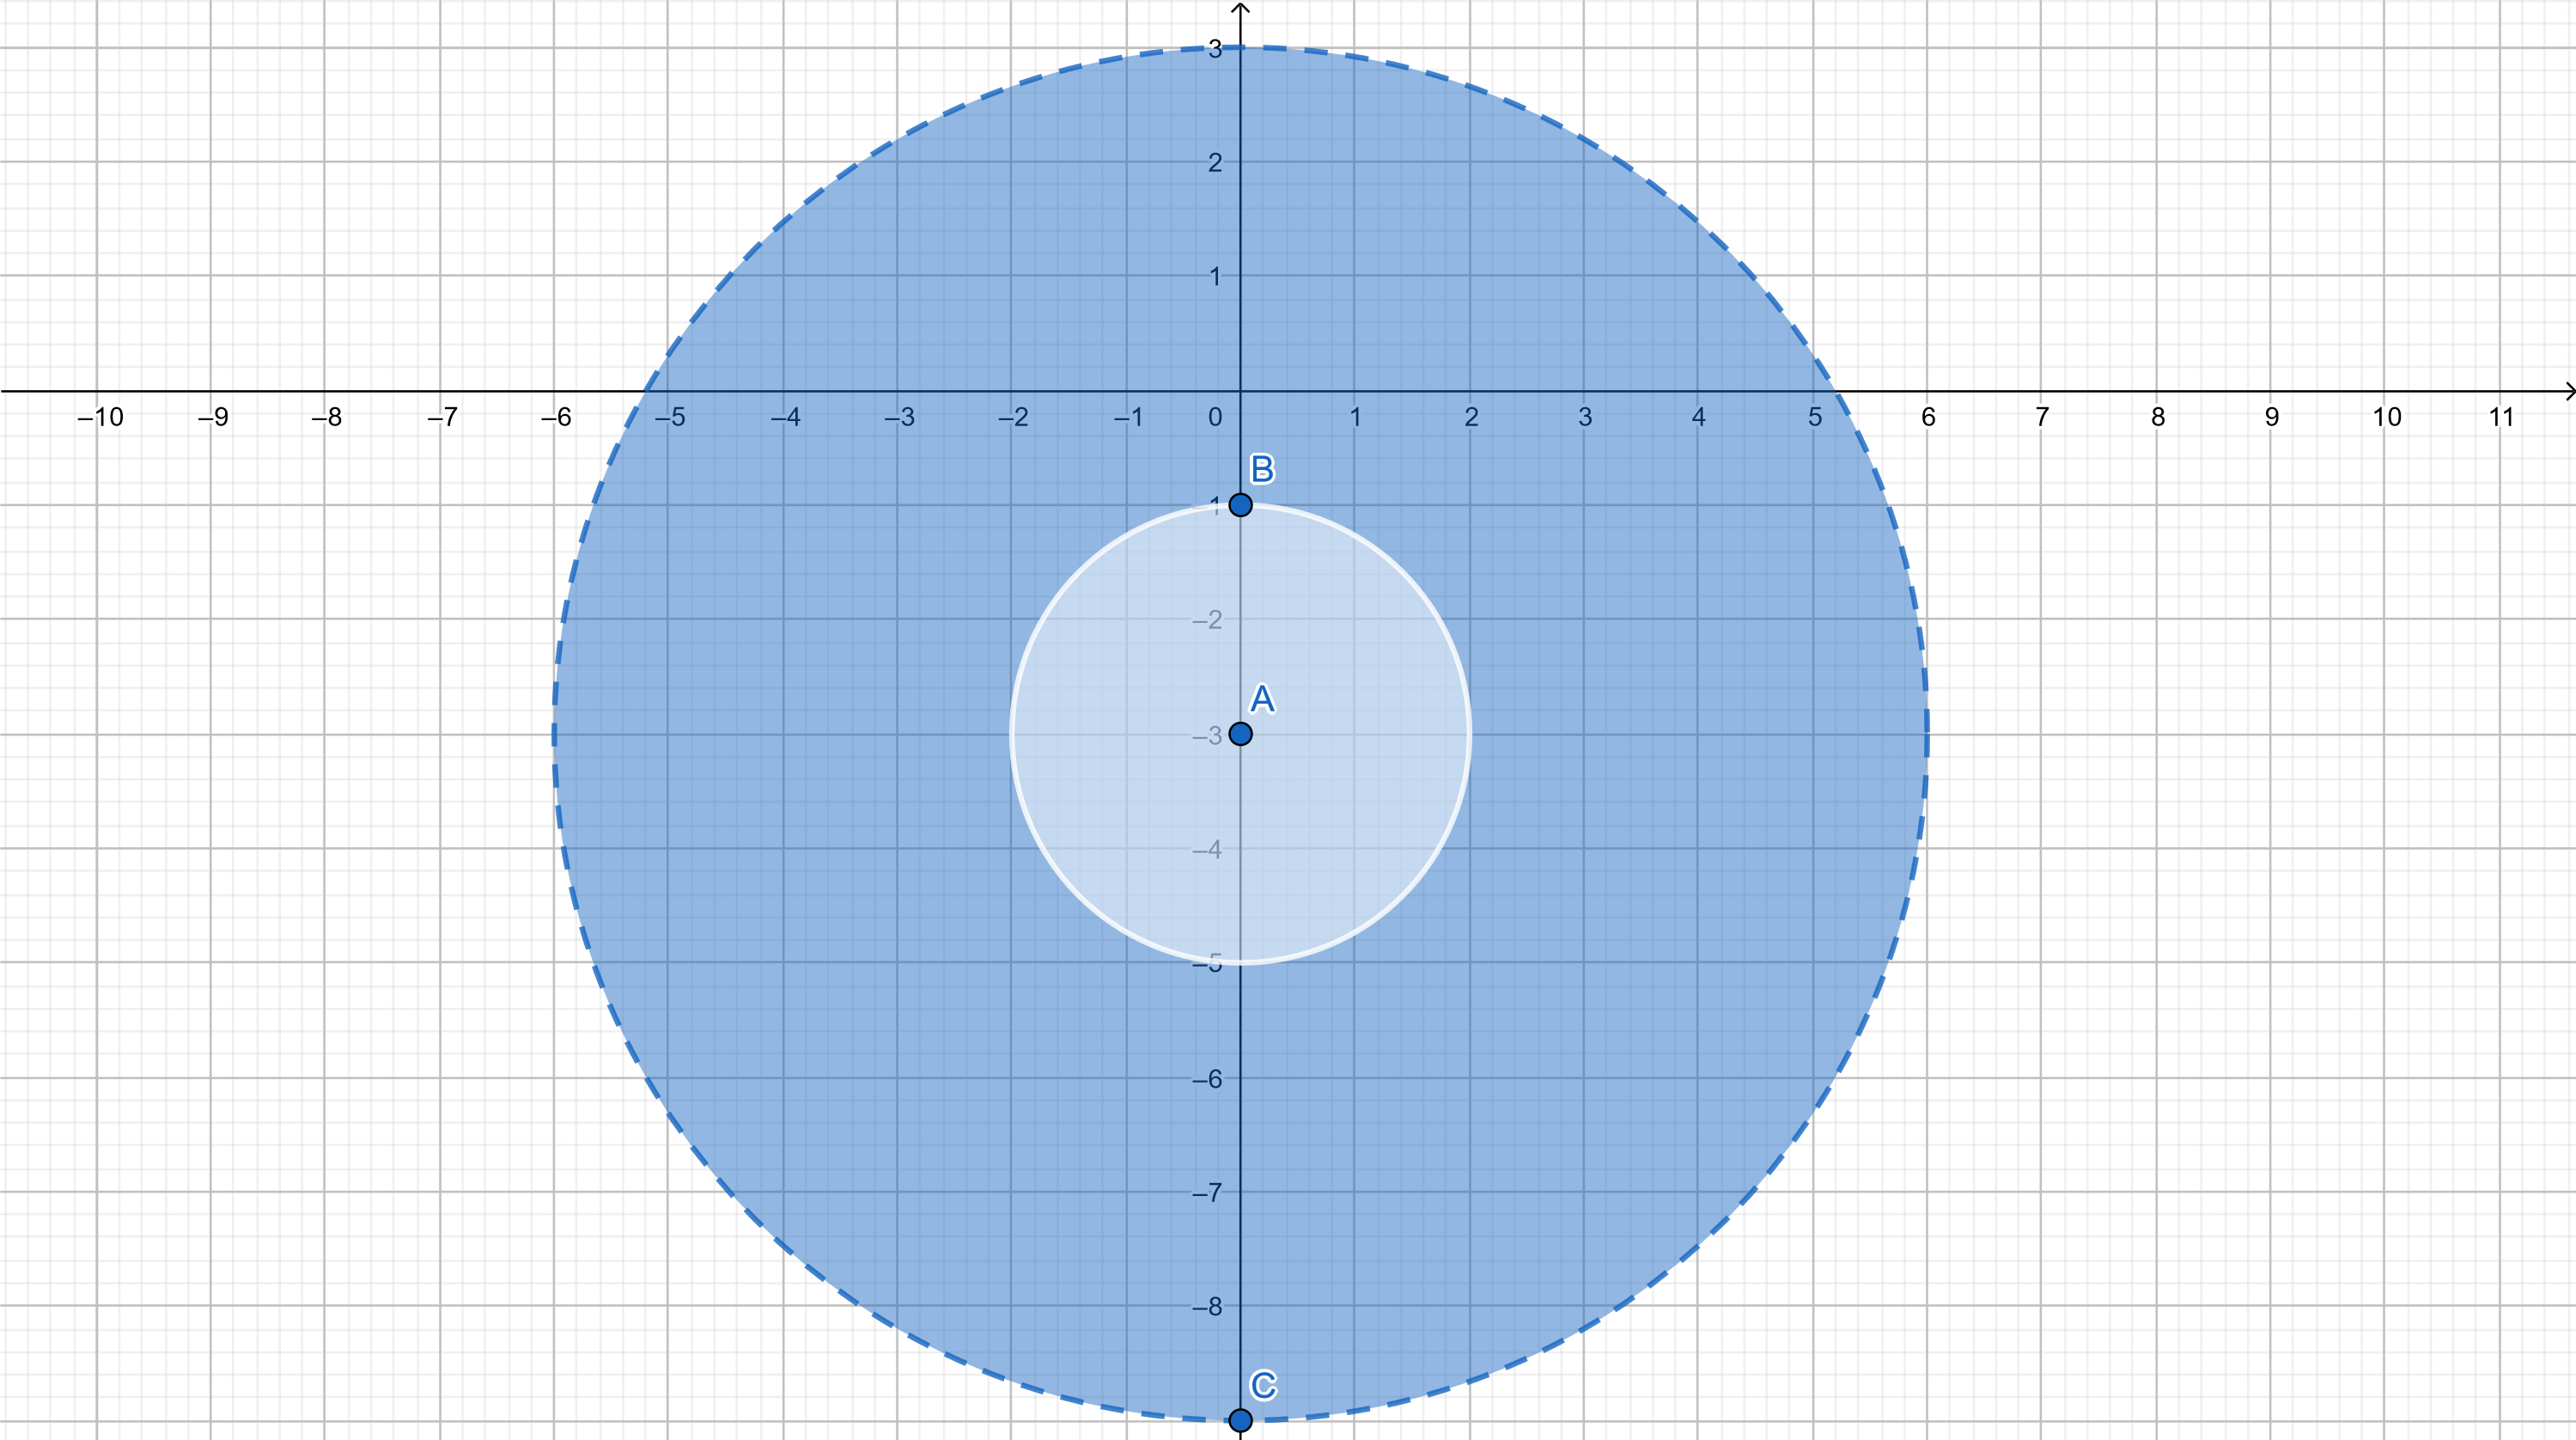
\includegraphics[width=10cm]{Gra-Ej-3.png}
\end{center}

\textcolor{ao(english)}{(\,4\,)} $\bf{2\,<\,|z\,+\,5\,-\,2\,i|\,<\,9}$.\\
$\text{Anillo abierto}$

El radio $r_{1}\,=\,2$ y $r_{2}\,=\,9$ el centro de este es $z_{0}\,=-\,5\,+\,2\,i$.\\

\begin{center}
    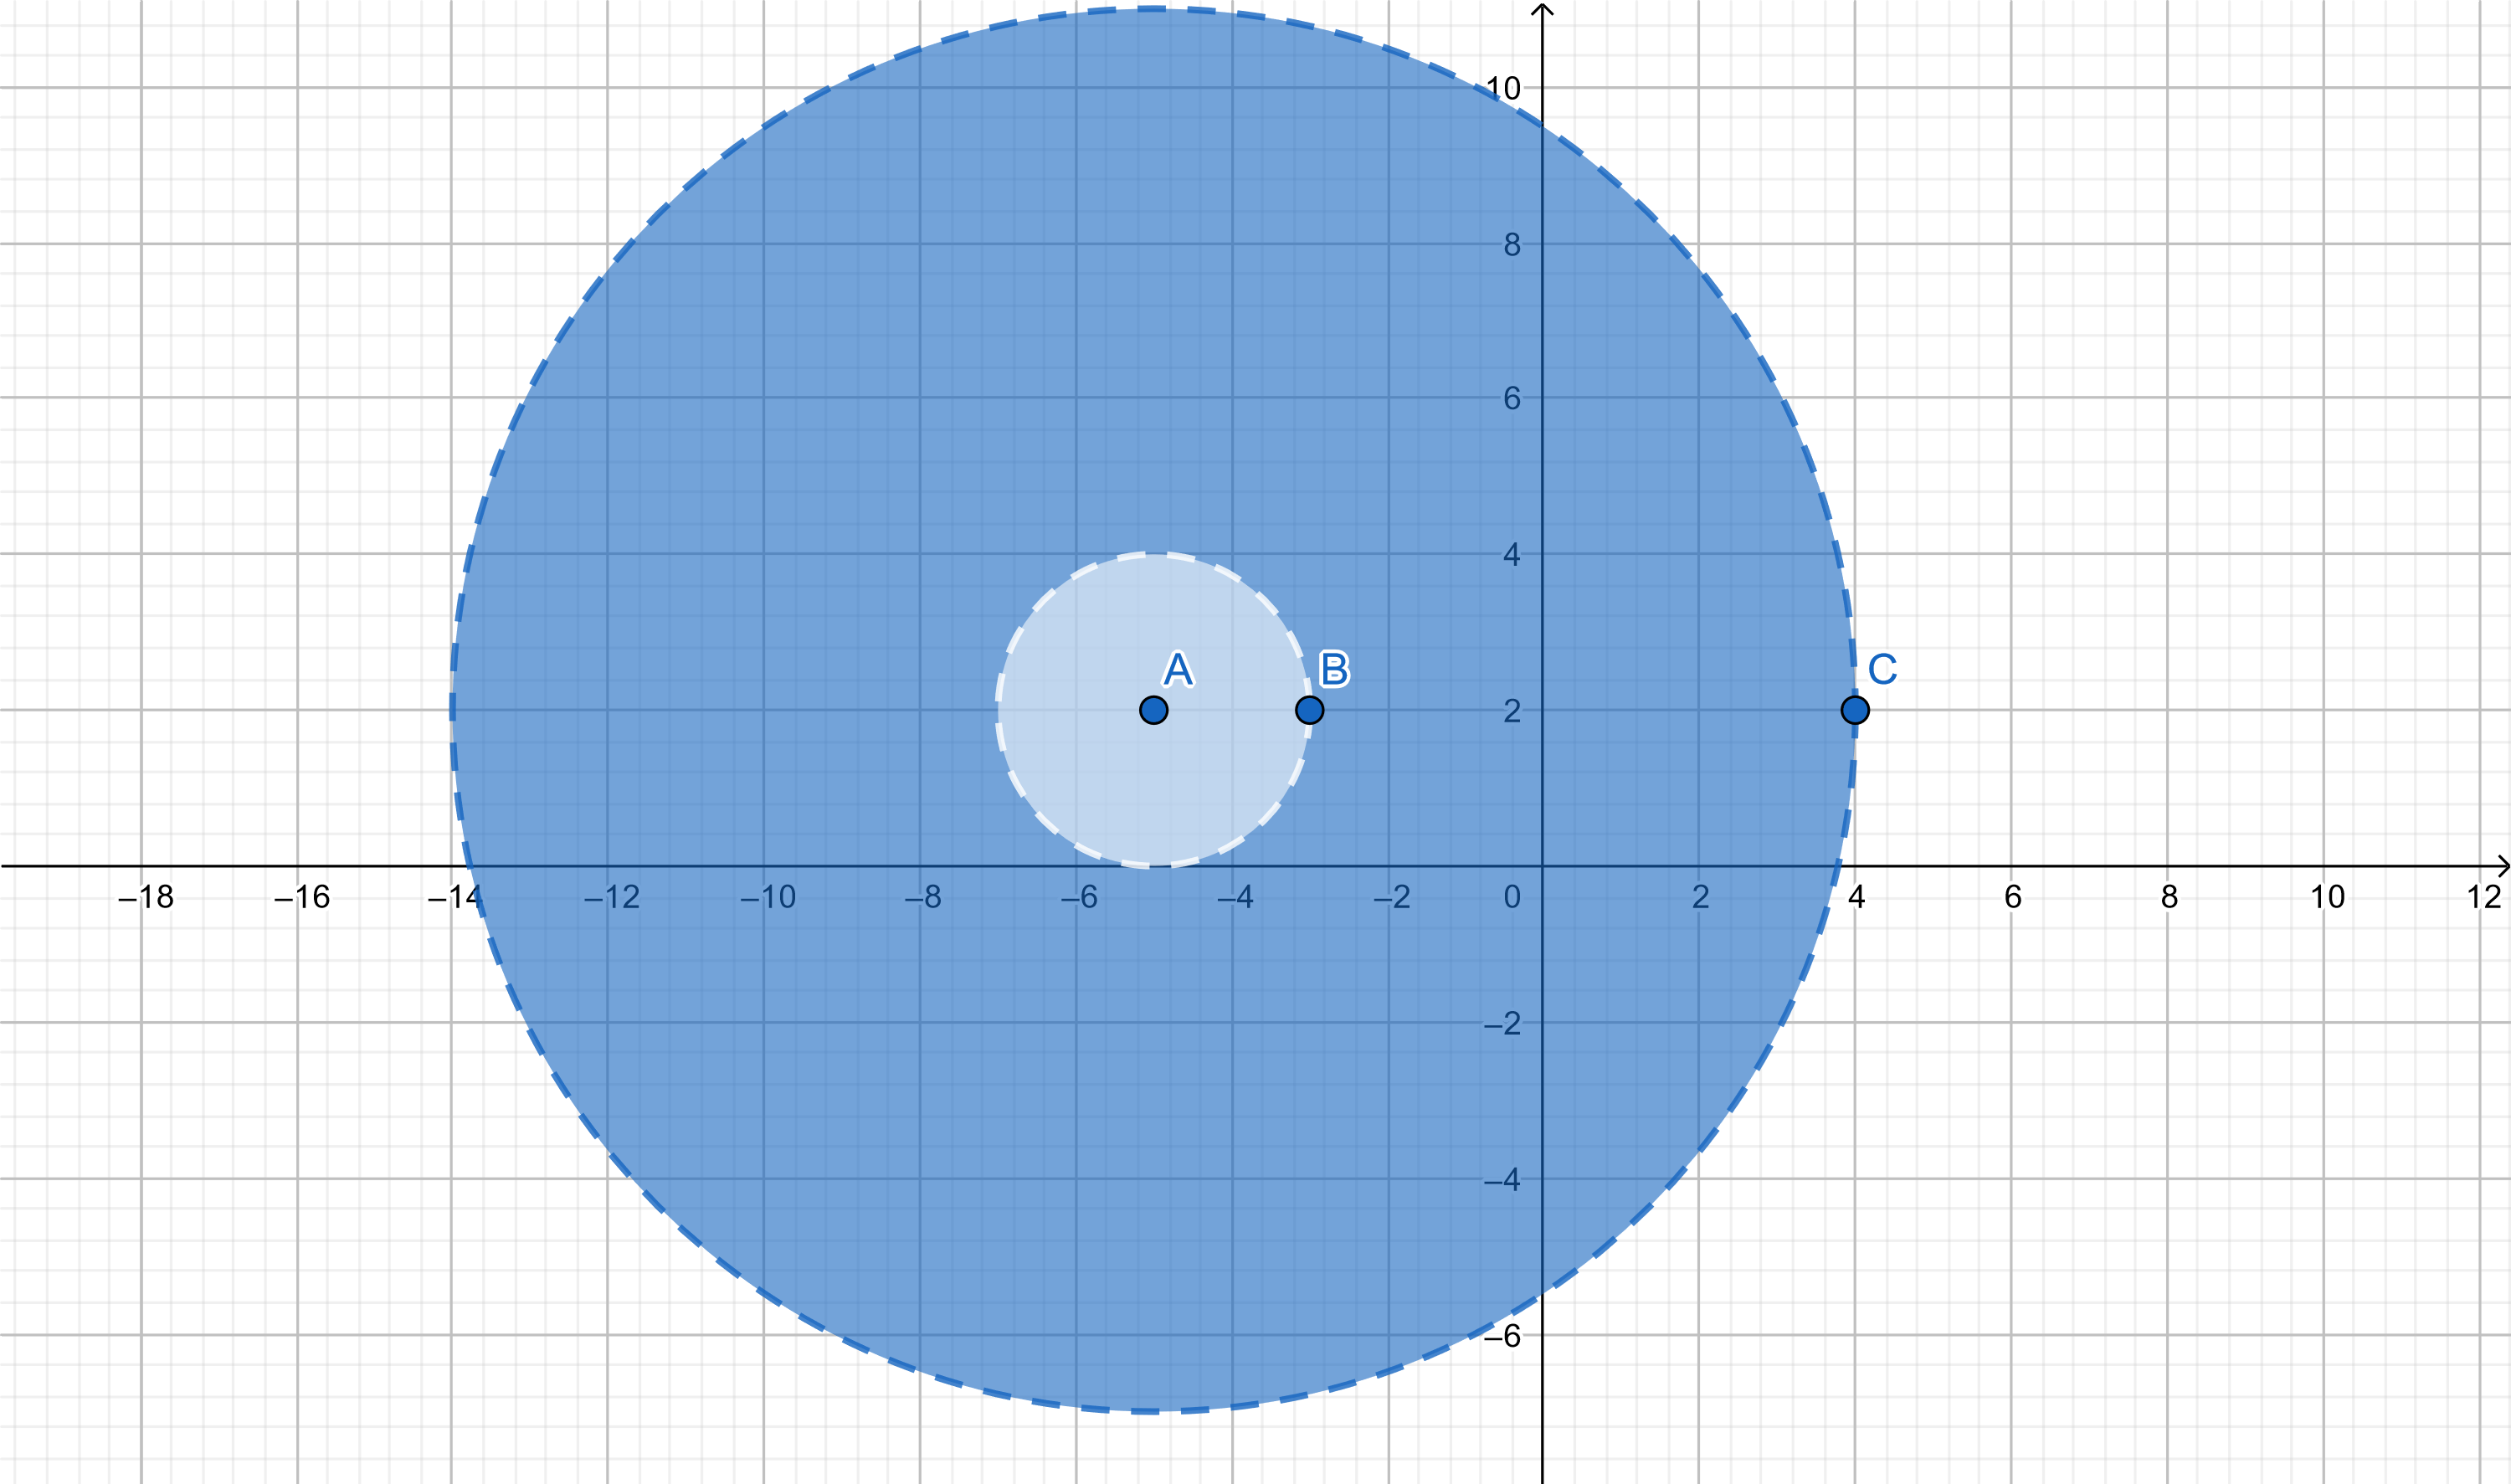
\includegraphics[width=10cm]{Gra-Ej-4.png}
\end{center}

\textcolor{ao(english)}{(\,5\,)} $\bf{|z\,-\,4\,+\,8\,i|\,<\,\dfrac{7}{2}}$.

$$|z\,-\,4\,+\,8\,i|\,<\,\dfrac{7}{2} \quad\iff\quad |z\,-\,(4\,-\,8\,i)|\,<\,\dfrac{7}{2}$$

El radio del Disco Abierto (\underline{Vecindad}) es $r\,=\,7\,/\,2$ y el centro de este es $z_{0}\,=\,4\,-\,8\,i$.\\

\textcolor{ao(english)}{\ding{47}} Graficar la Vecindad.

\begin{center}
    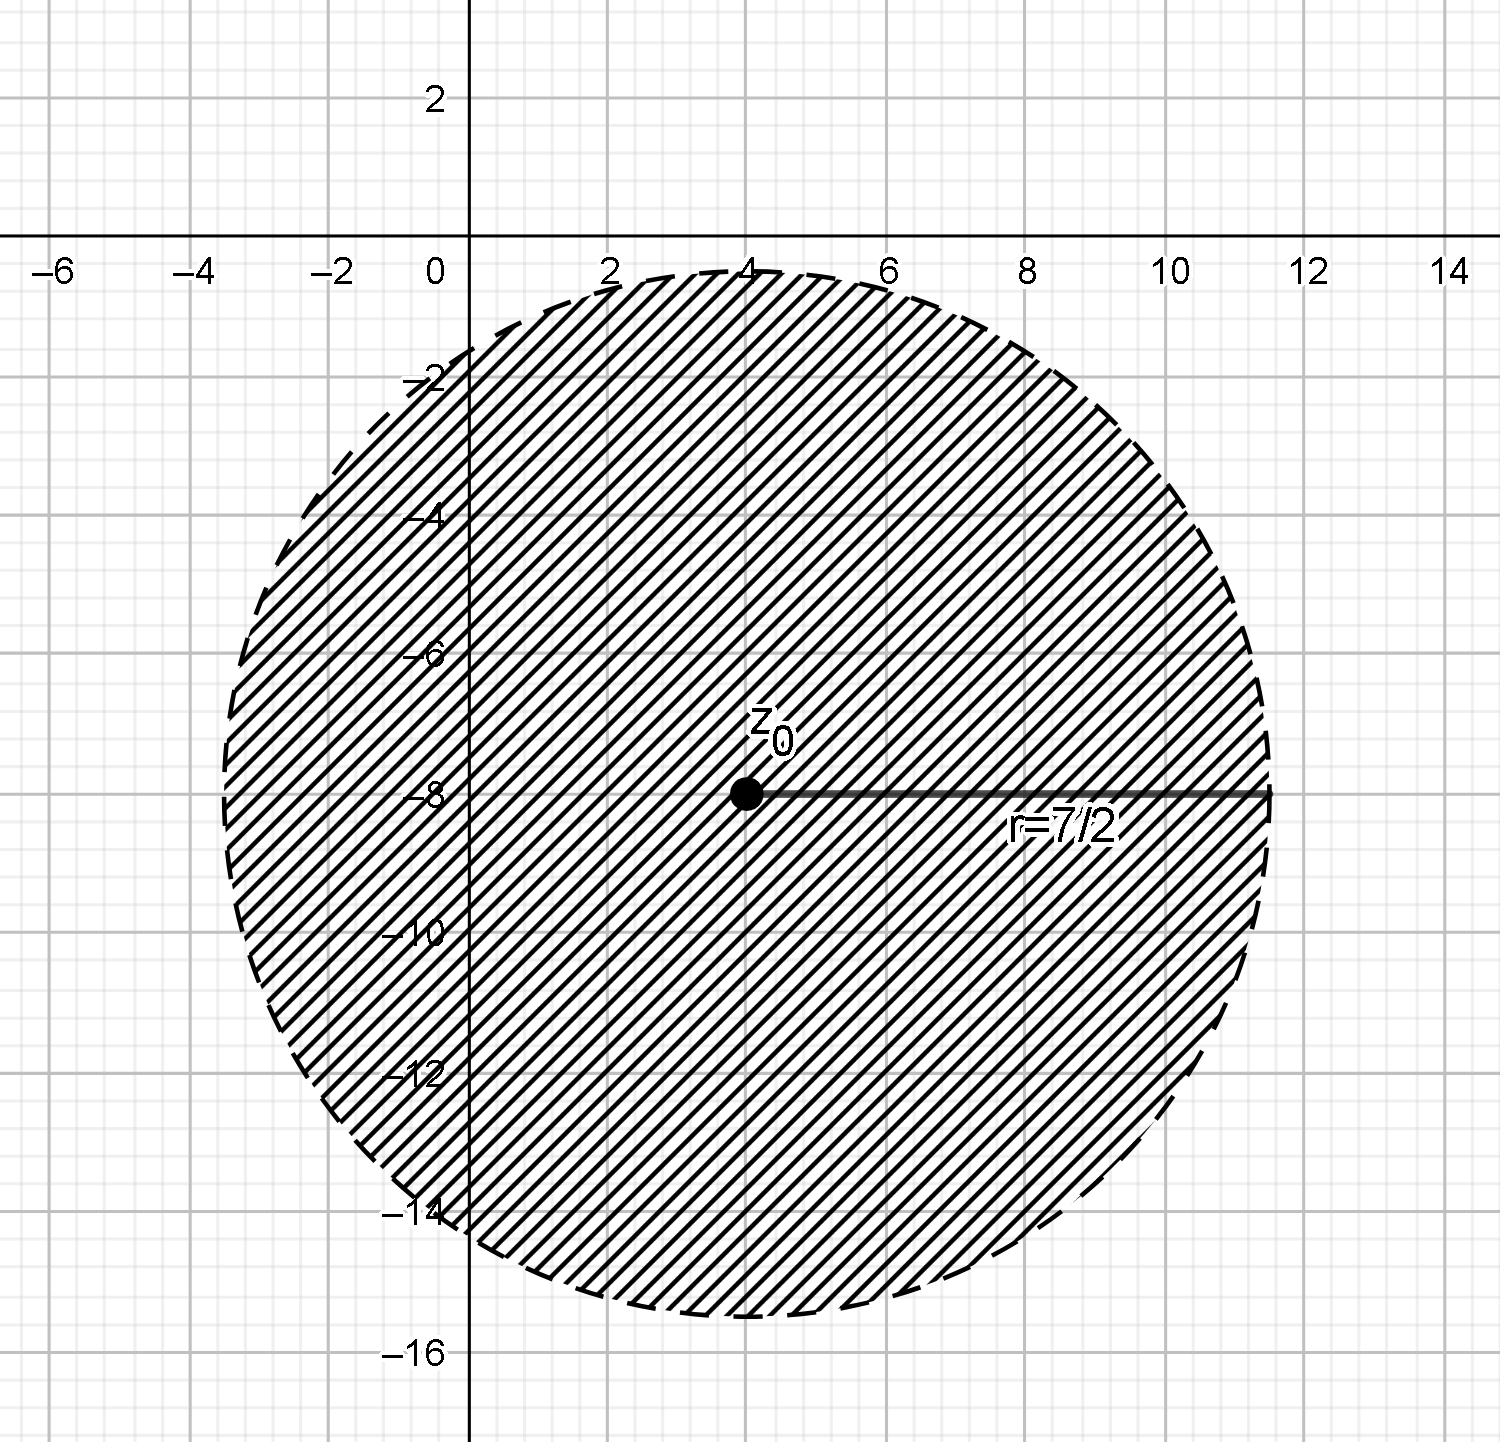
\includegraphics[width=10cm]{Gra-Ej-5.png}
\end{center}

\textcolor{ao(english)}{(\,6\,)} $\bf{|z\,+\,4\,+\,2\,i|\,=\,6}$.

$$|z\,+\,4\,+\,2\,i|\,=\,6 \quad\iff\quad |z\,-\,(-\,4\,-\,2\,i)|\,<\,6$$

El radio del Círculo es $r\,=\,6$ y el centro de este es $z_{0}\,=\,-\,4\,-\,2\,i$.\\

\textcolor{ao(english)}{\ding{47}} Graficar el Círculo.

\begin{center}
     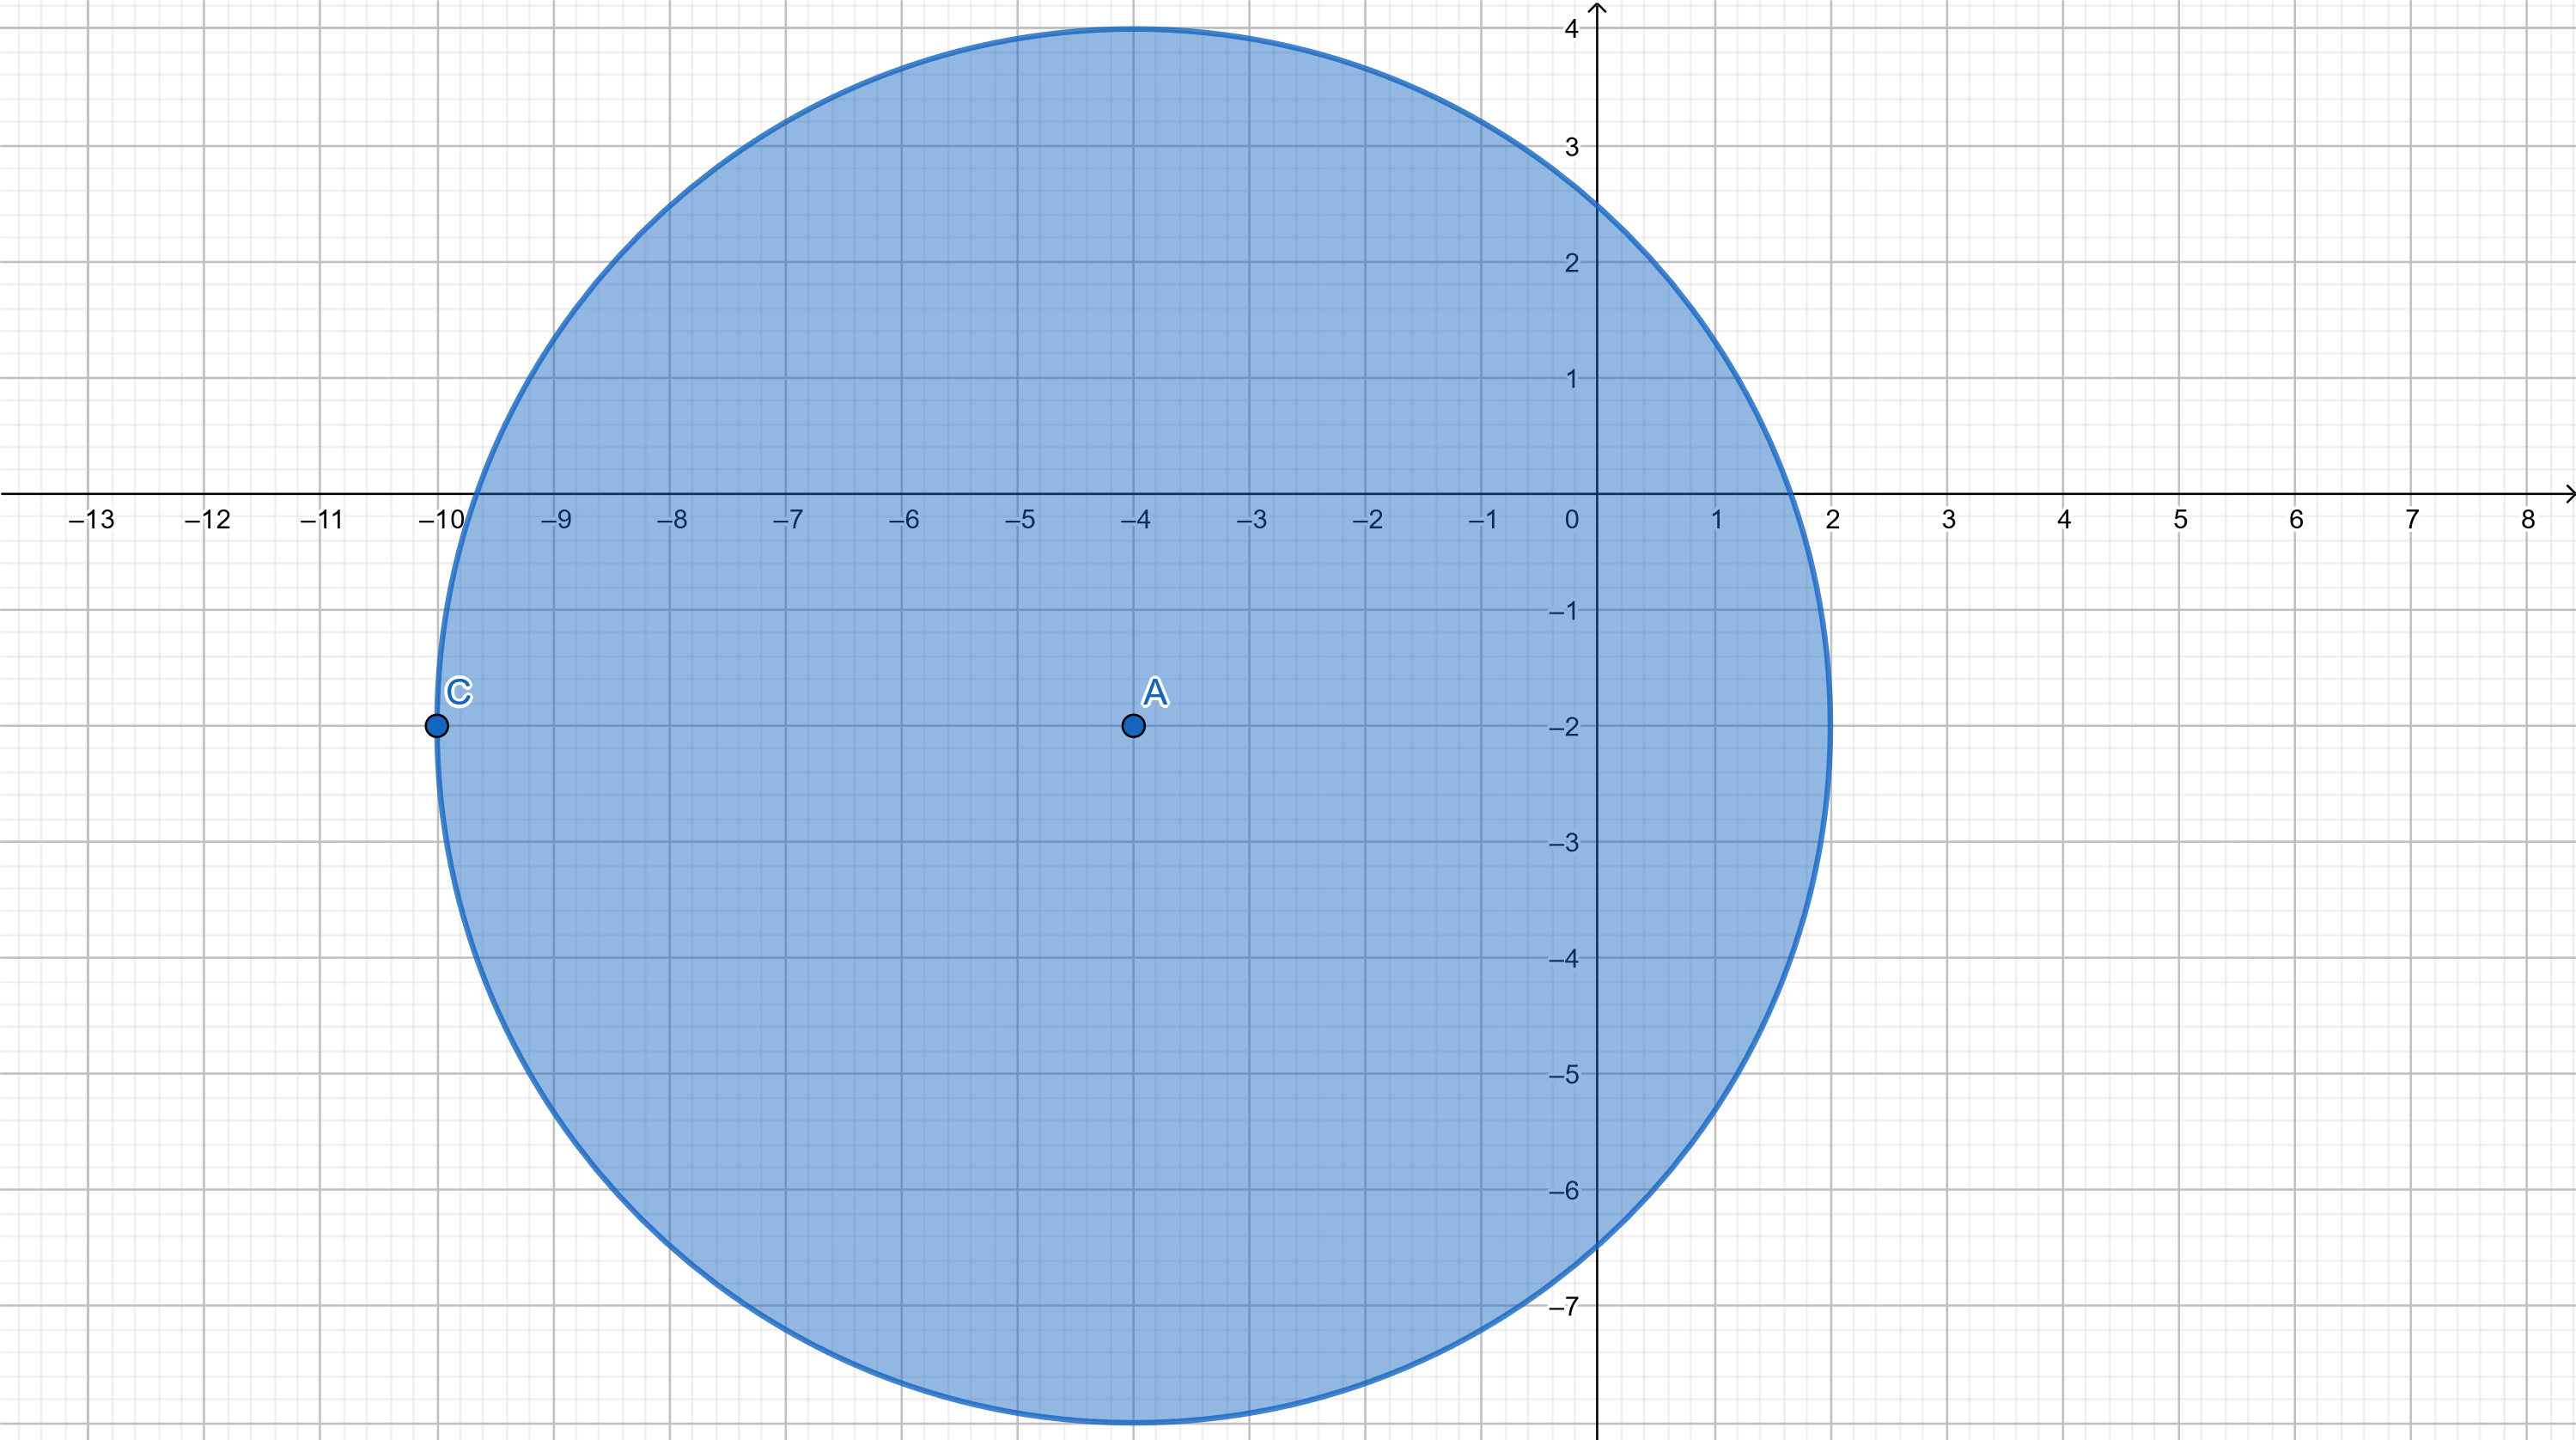
\includegraphics[width=10cm]{Gra-Ej-6.png}
\end{center}

\textcolor{ao(english)}{(\,7\,)} $\bf{0\,<\,|z\,-\,1\,+\,4\,i|\,\leq\,5}$.

$$0\,<\,|z\,-\,1\,+\,4\,i|\,\leq\,5 \quad\iff\quad 0\,<\,|z\,-\,(1\,-\,4\,i)|\,\leq\,5$$

El radio de la Vecindad Suprimida es $r\,=\,r_{2}\,=\,5$; ya que $r_{1}\,=\,0$ y el centro de este es $z_{0}\,=\,1\,-\,4\,i$.\\

\textcolor{ao(english)}{\ding{47}} Graficar la Vecindad Suprimida.

\begin{center}
    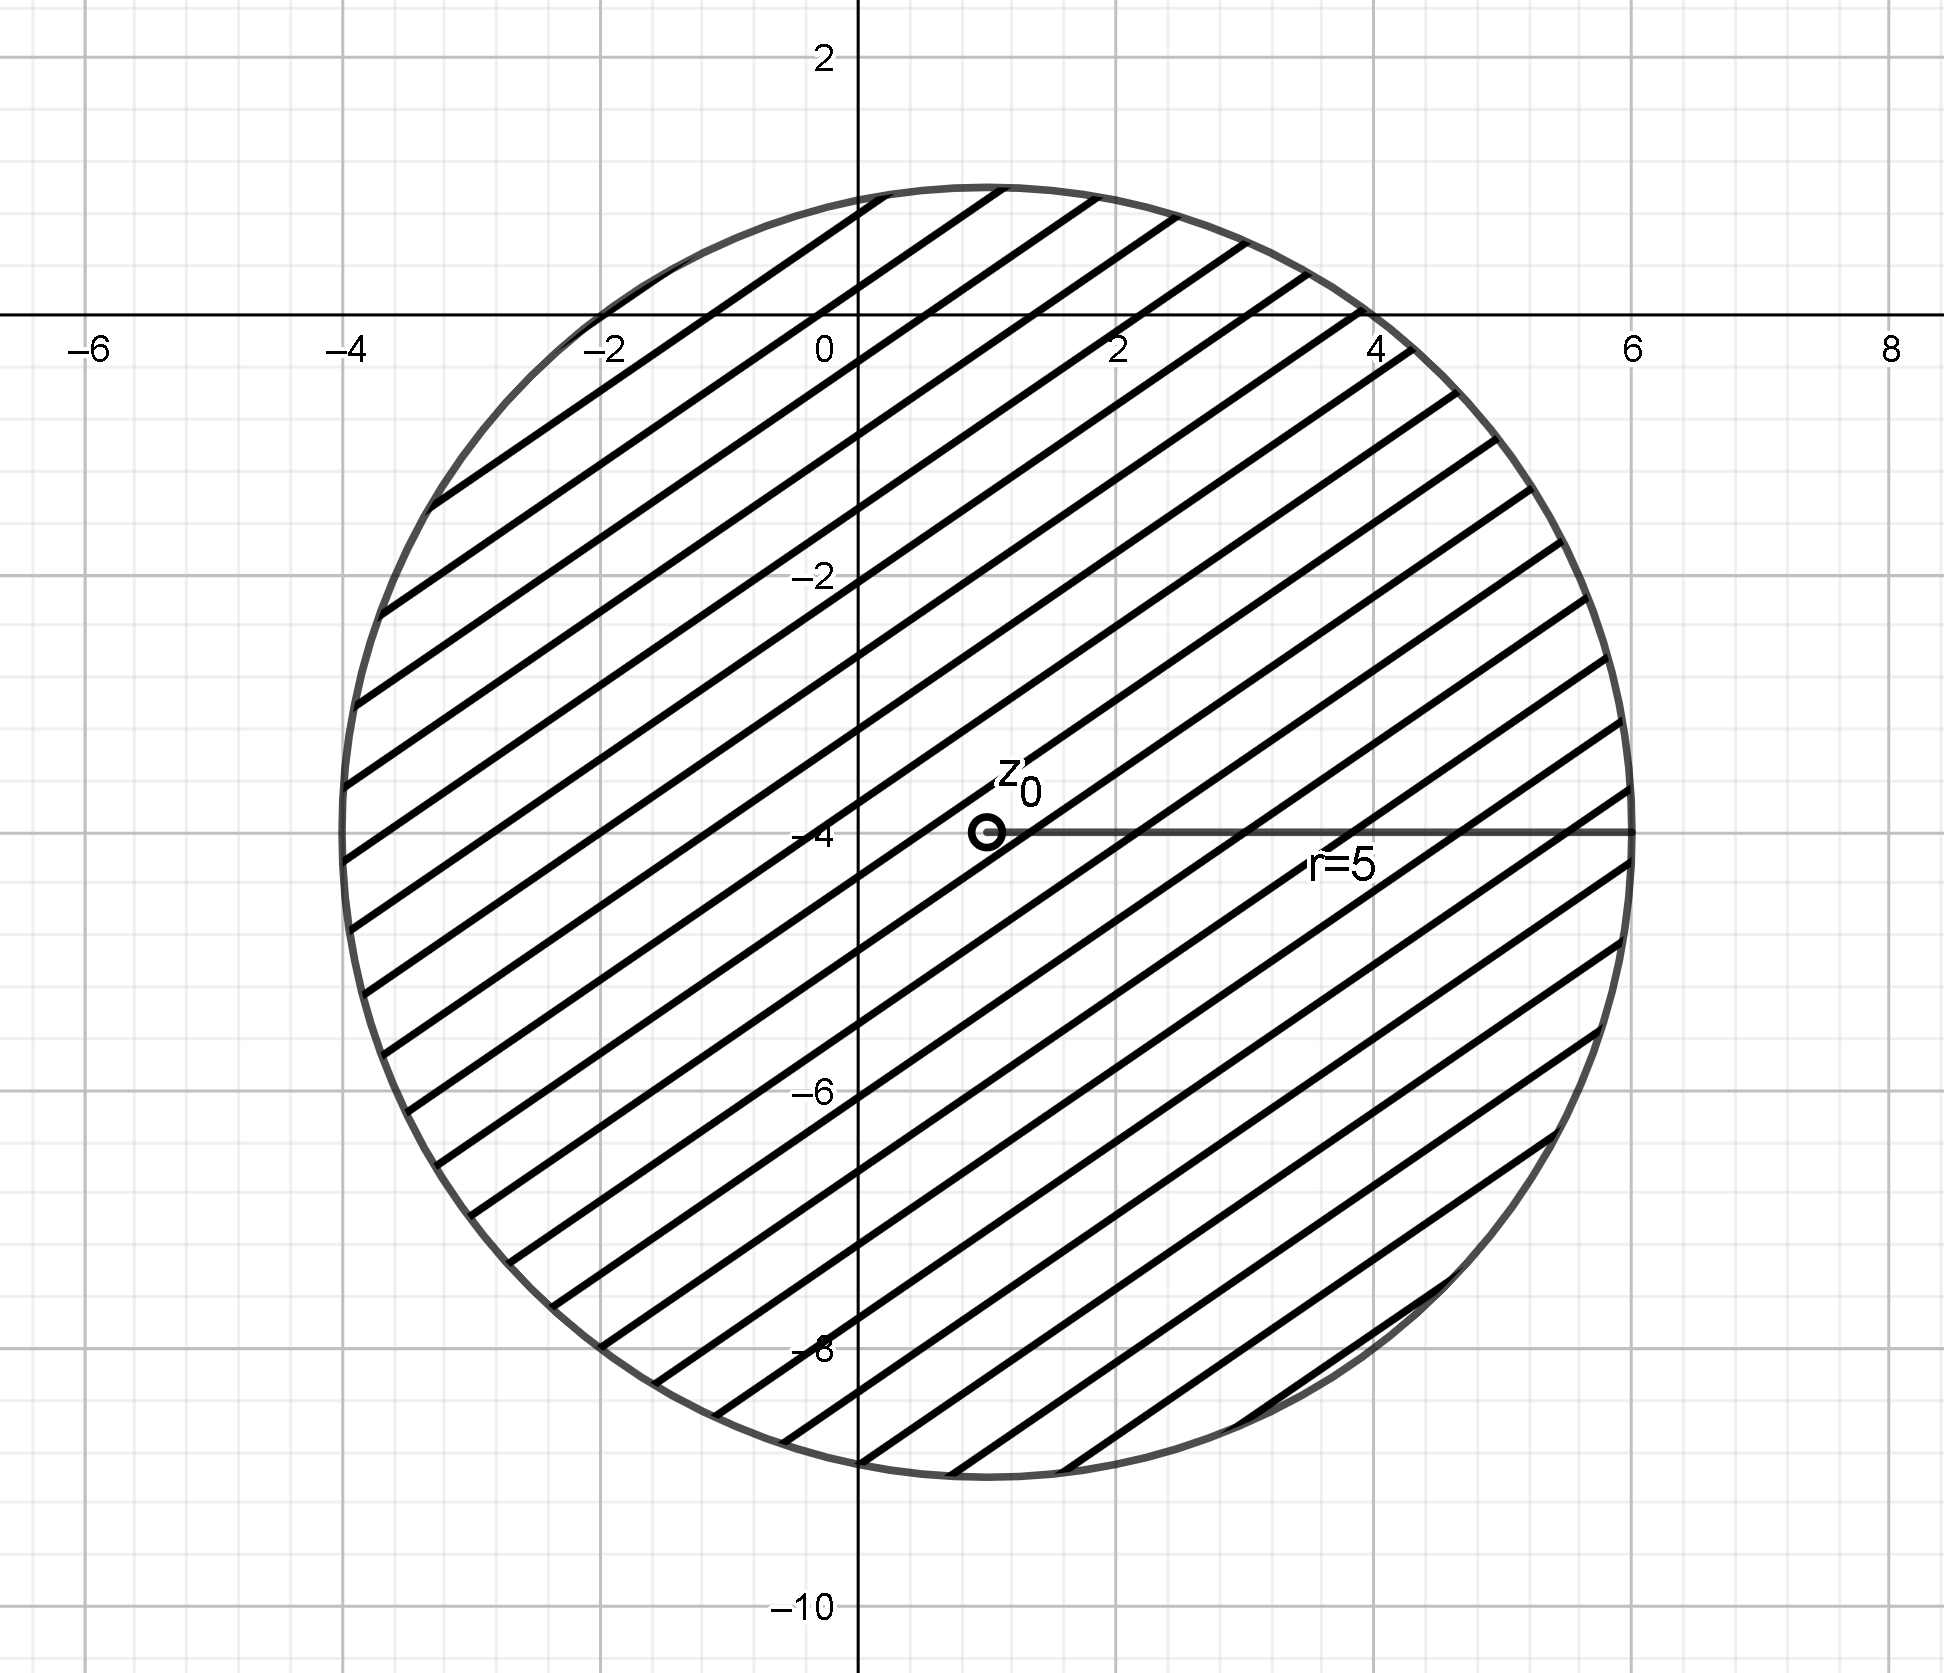
\includegraphics[width=10cm]{Gra-Ej-7.png}
\end{center}

\textcolor{ao(english)}{(\,8\,)} $\bf{2\,\leq\,|z\,-\,1|\,\leq\,9}$.\\
$\text{Anillo cerrado}$

El radio $r_{1}\,=\,2$ y $r_{2}\,=\,9$ el centro de este es $z_{0}\,=\,1\,i$.\\

\begin{center}
    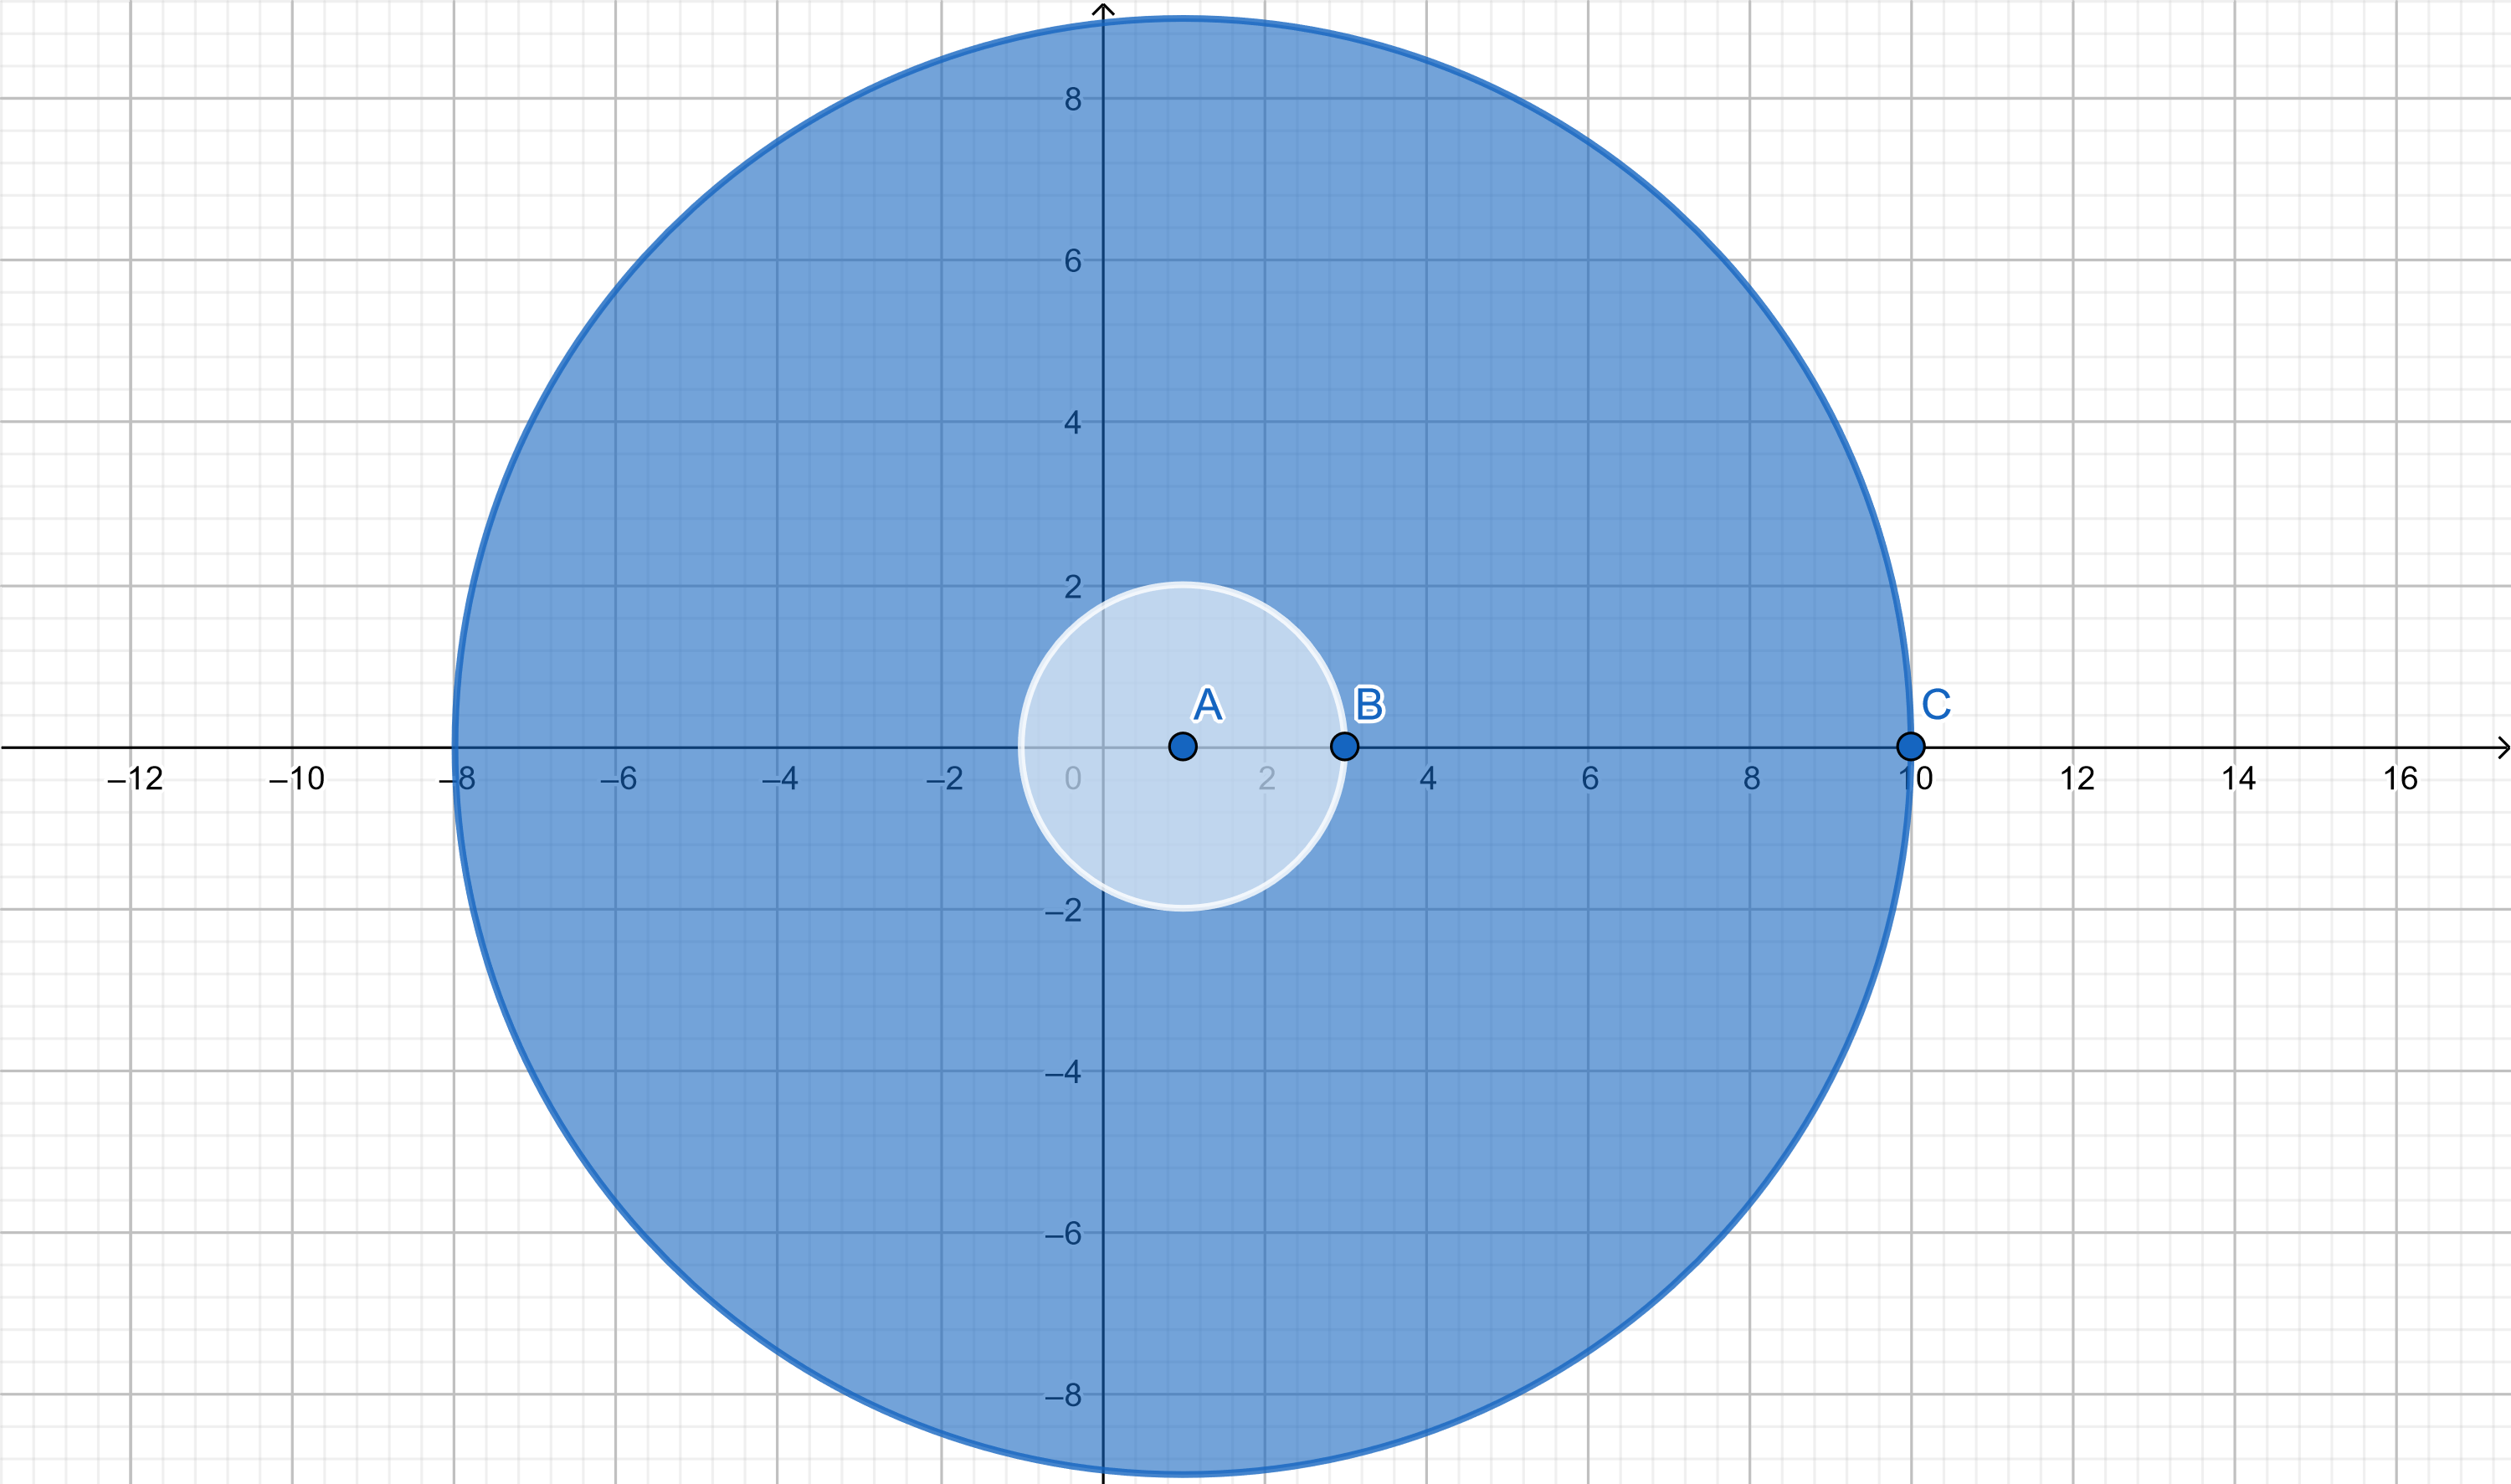
\includegraphics[width=10cm]{Gra-Ej-8.png}
\end{center}

\textcolor{ao(english)}{(\,9\,)} $\bf{\mathnormal{Im}\,(\overline{z}\,+\,3\,i)\,=\,6}$.

$$z\,=\,x\,+\,i\,y \quad\iff\quad \overline{z}\,=\,x\,-\,i\,y $$

$$\overline{z}\,+\,3\,i\,=\,x\,-\,i\,y\,+\,3\,i\,=\,x\,+(\,-\,y\,+\,3\,)\,i$$

$$\mathnormal{Im}\,(\overline{z}\,+\,3\,i)\,=\,-\,y\,+\,3$$.

$$-\,y\,+\,3\,=\,6 \quad\iff\quad y\,=\,-\,3$$

\begin{center}
    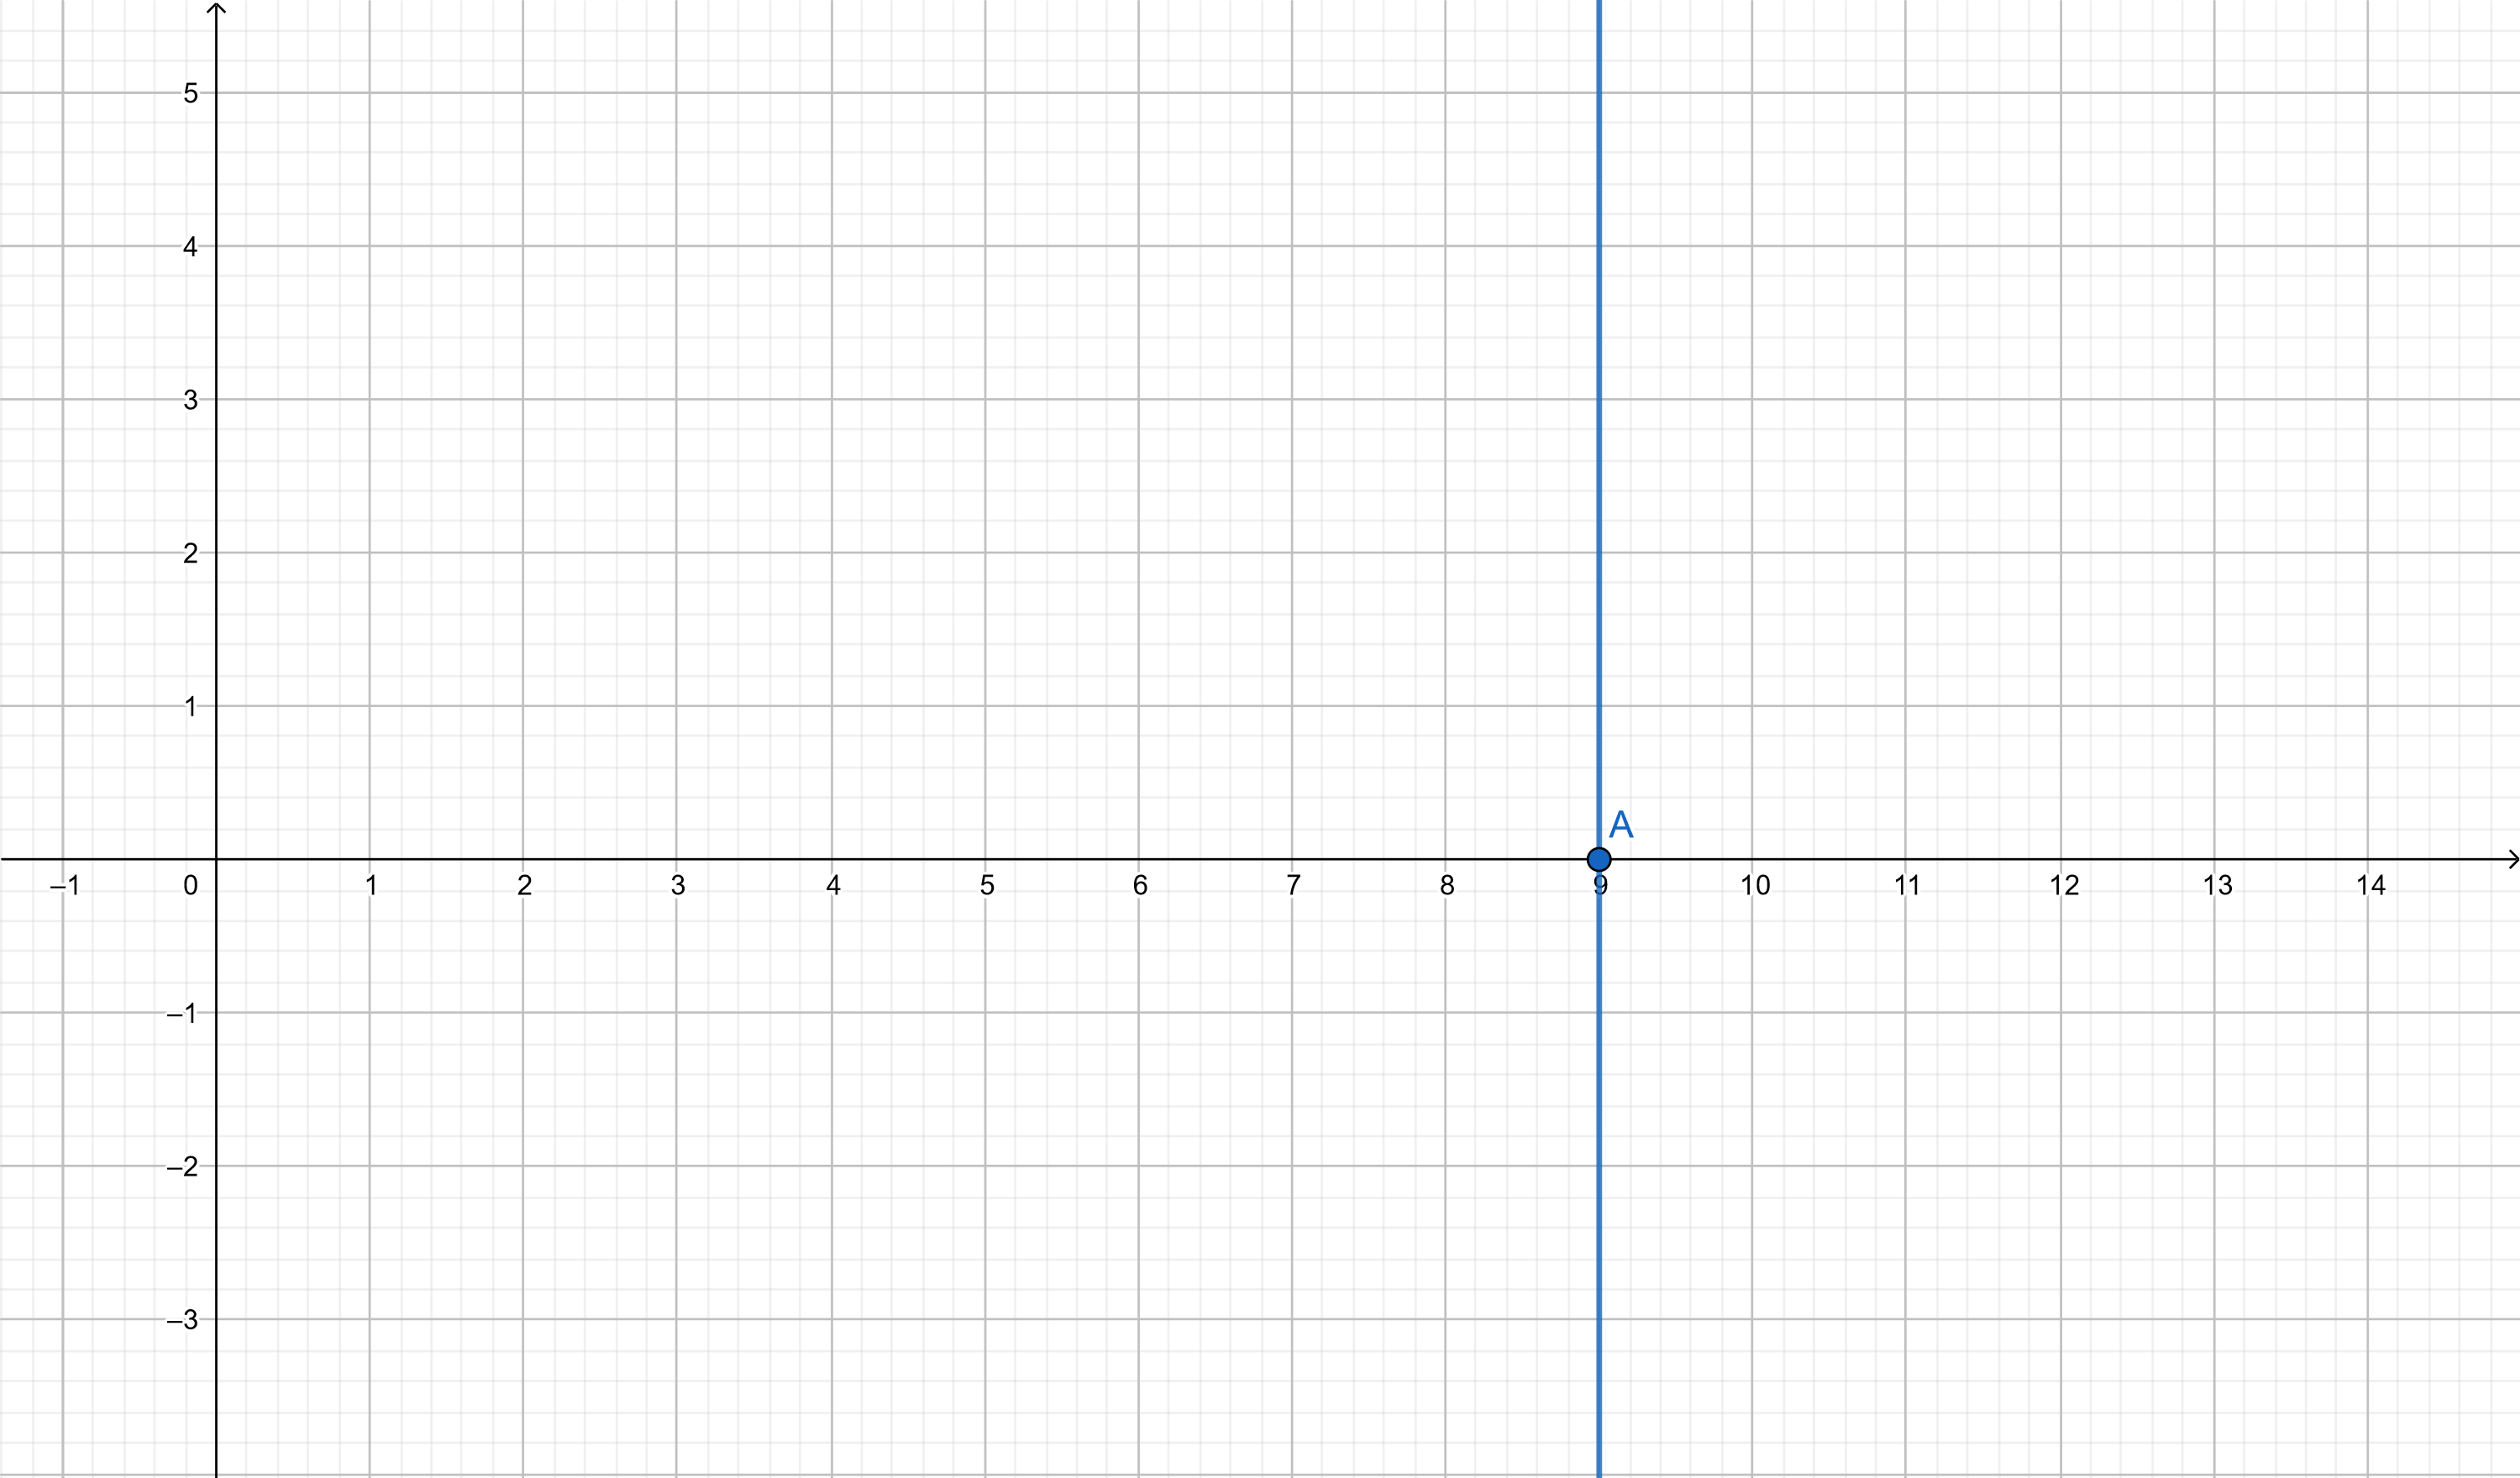
\includegraphics[width=10cm]{Gra-Ej-9.png}
\end{center}

\textcolor{ao(english)}{(\,10\,)} $\bf{\mathnormal{Re}\,(z\,+\,8)\,=\,5}$.\\


Asintota con valor de $5$.\\

\begin{center}
    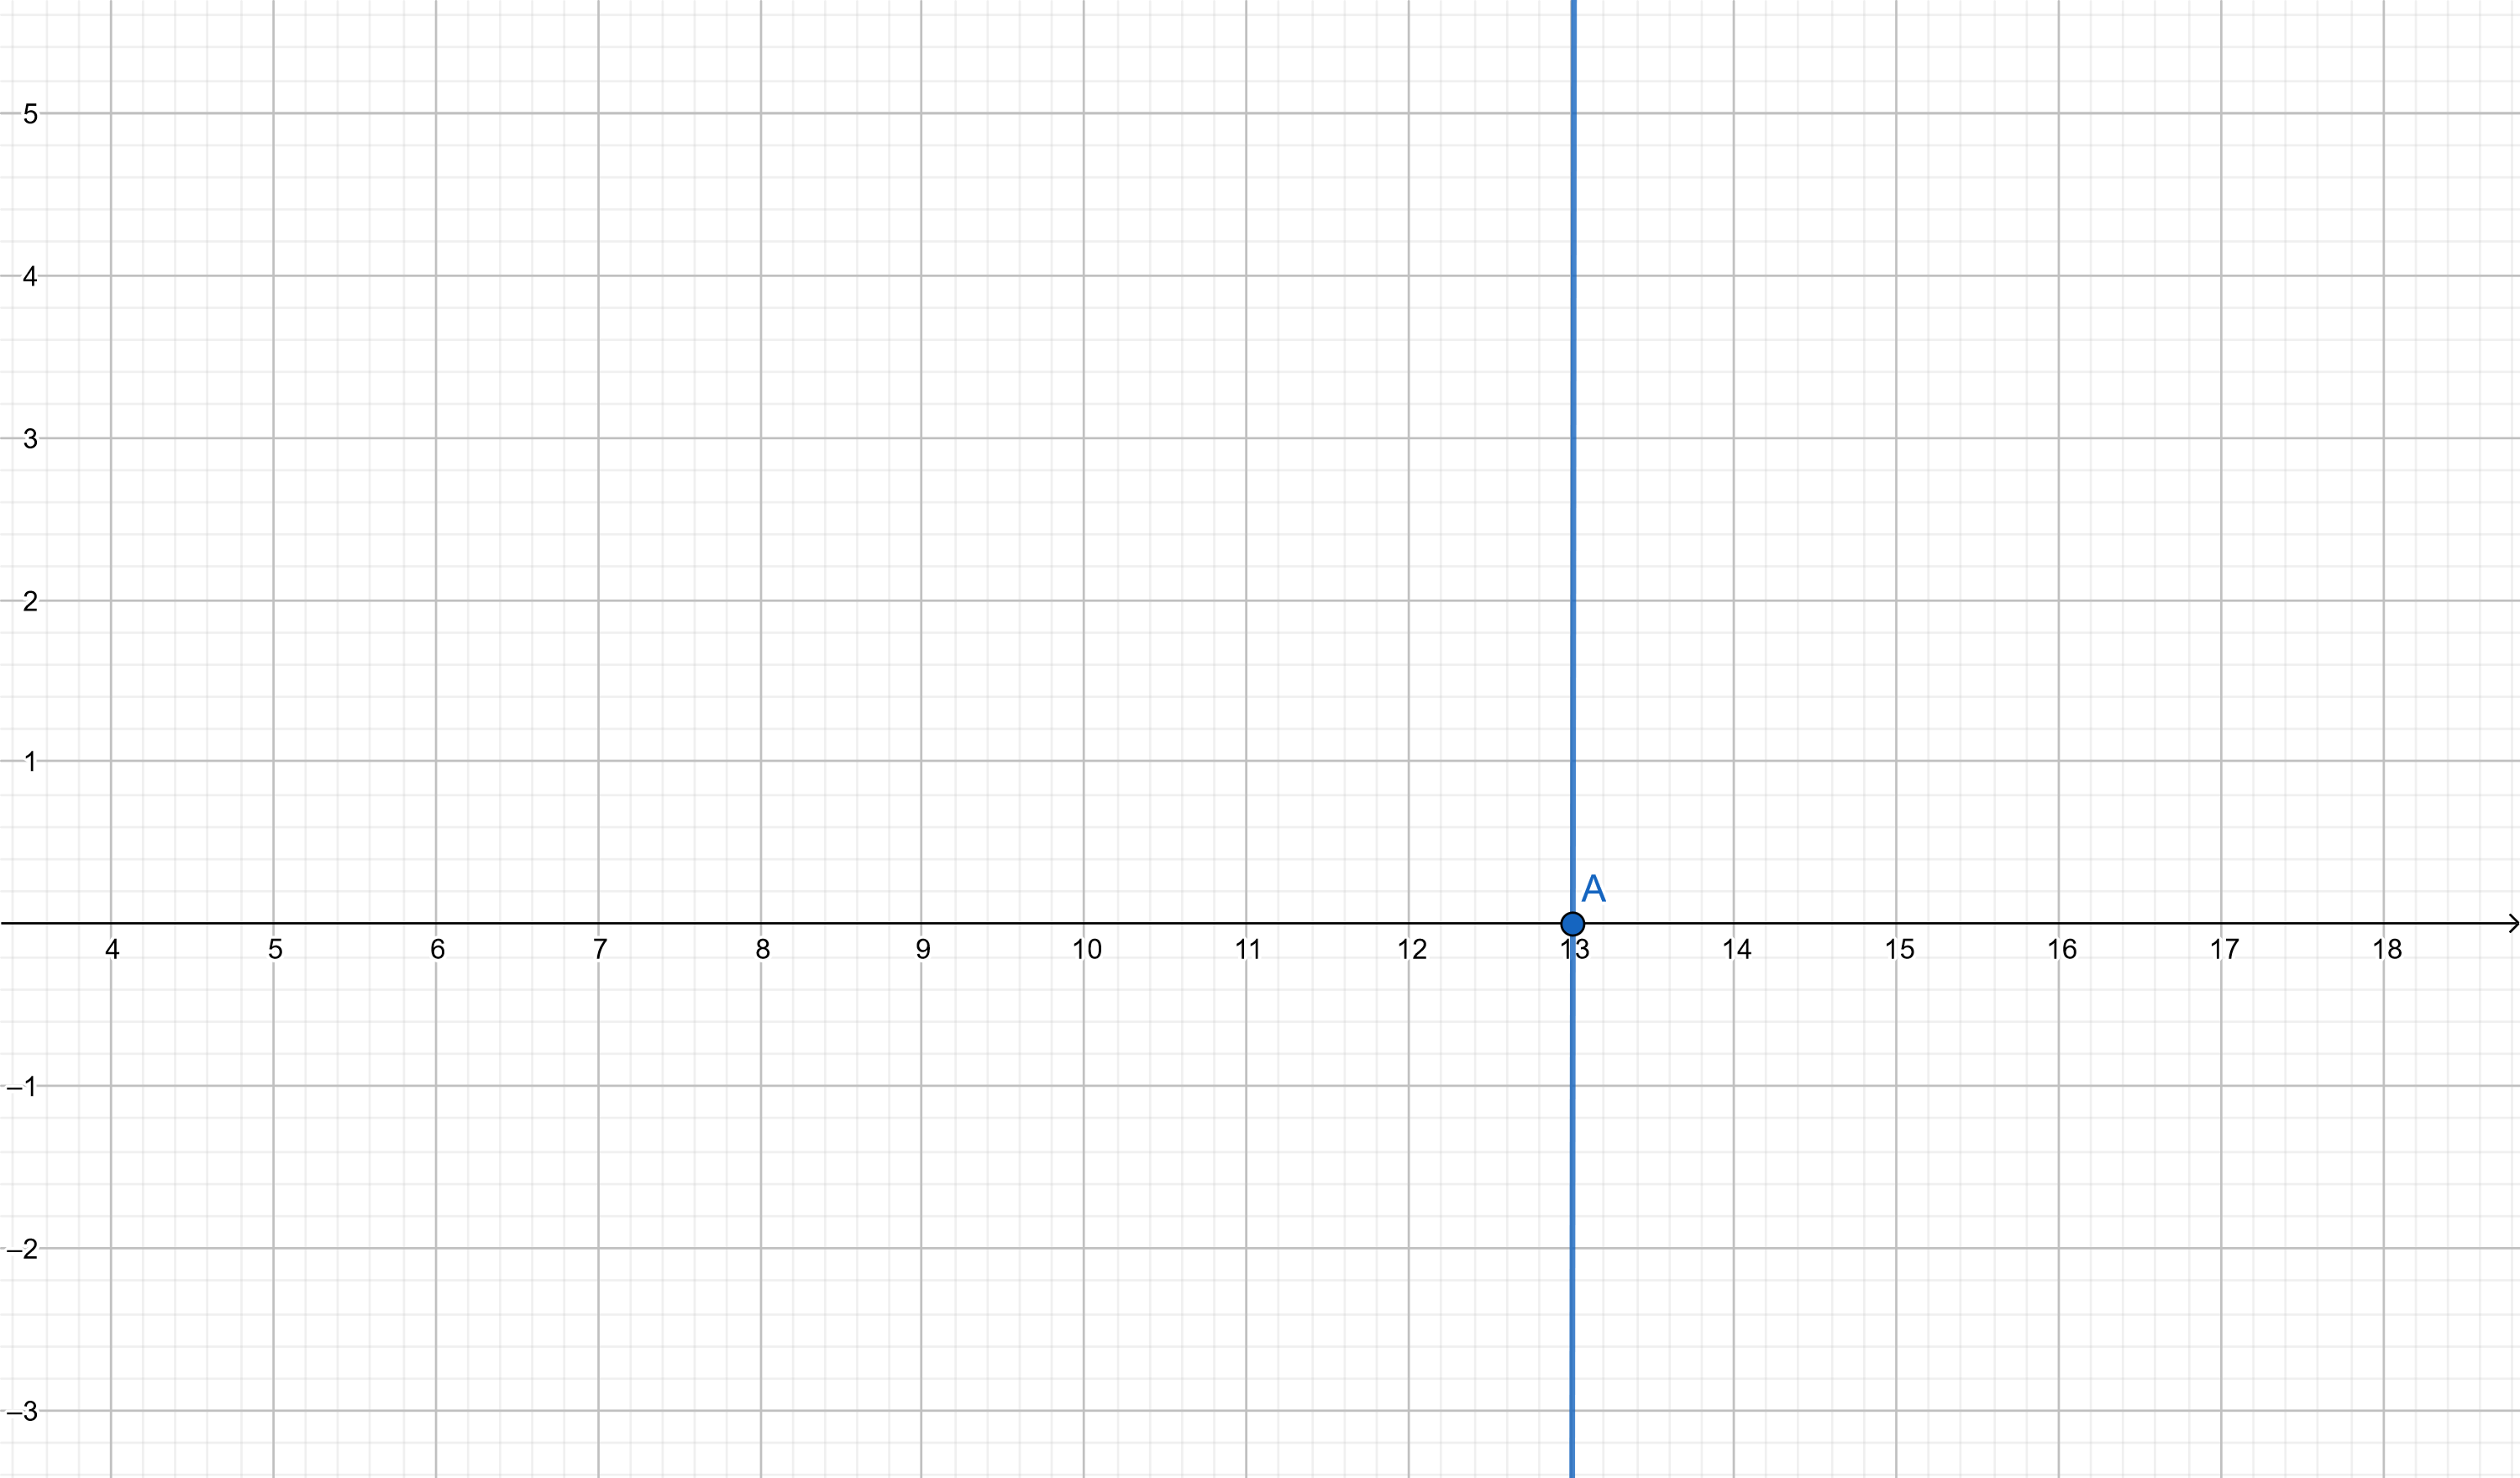
\includegraphics[width=10cm]{Gra-Ej-10.png}
\end{center}

\textcolor{ao(english)}{(\,11\,)} $\bf{\mathnormal{Im}\,(z\,-\,10\,+\,2\,i)\,>\,\dfrac{5}{4}}$.

$$\mathnormal{Im}\,(z\,-\,10\,+\,2\,i)\,>\,\dfrac{5}{4} \quad\iff\quad \mathnormal{Im}\,(z\,-\,(10\,-\,2\,i))\,>\,\dfrac{5}{4} \quad\iff\quad \mathnormal{Im}\,(x\,+\,i\,y\,-\,(10\,-\,2\,i))\,>\,\dfrac{5}{4}$$

\textcolor{ao(english)}{\ding{47}} Solucinamos la parte $\mathnormal{Im}$ del conjunto.

$$y\,-\,2\,>\,\dfrac{5}{4} \quad\iff\quad y\,>\,\dfrac{5}{4}\,+\,2 \quad\iff\quad y\,>\,\dfrac{5\,+\,8}{4} \quad\iff\quad y\,>\,\dfrac{13}{4}$$

\textcolor{ao(english)}{\ding{47}} Graficar el Medio Plano Superior.

\begin{center}
    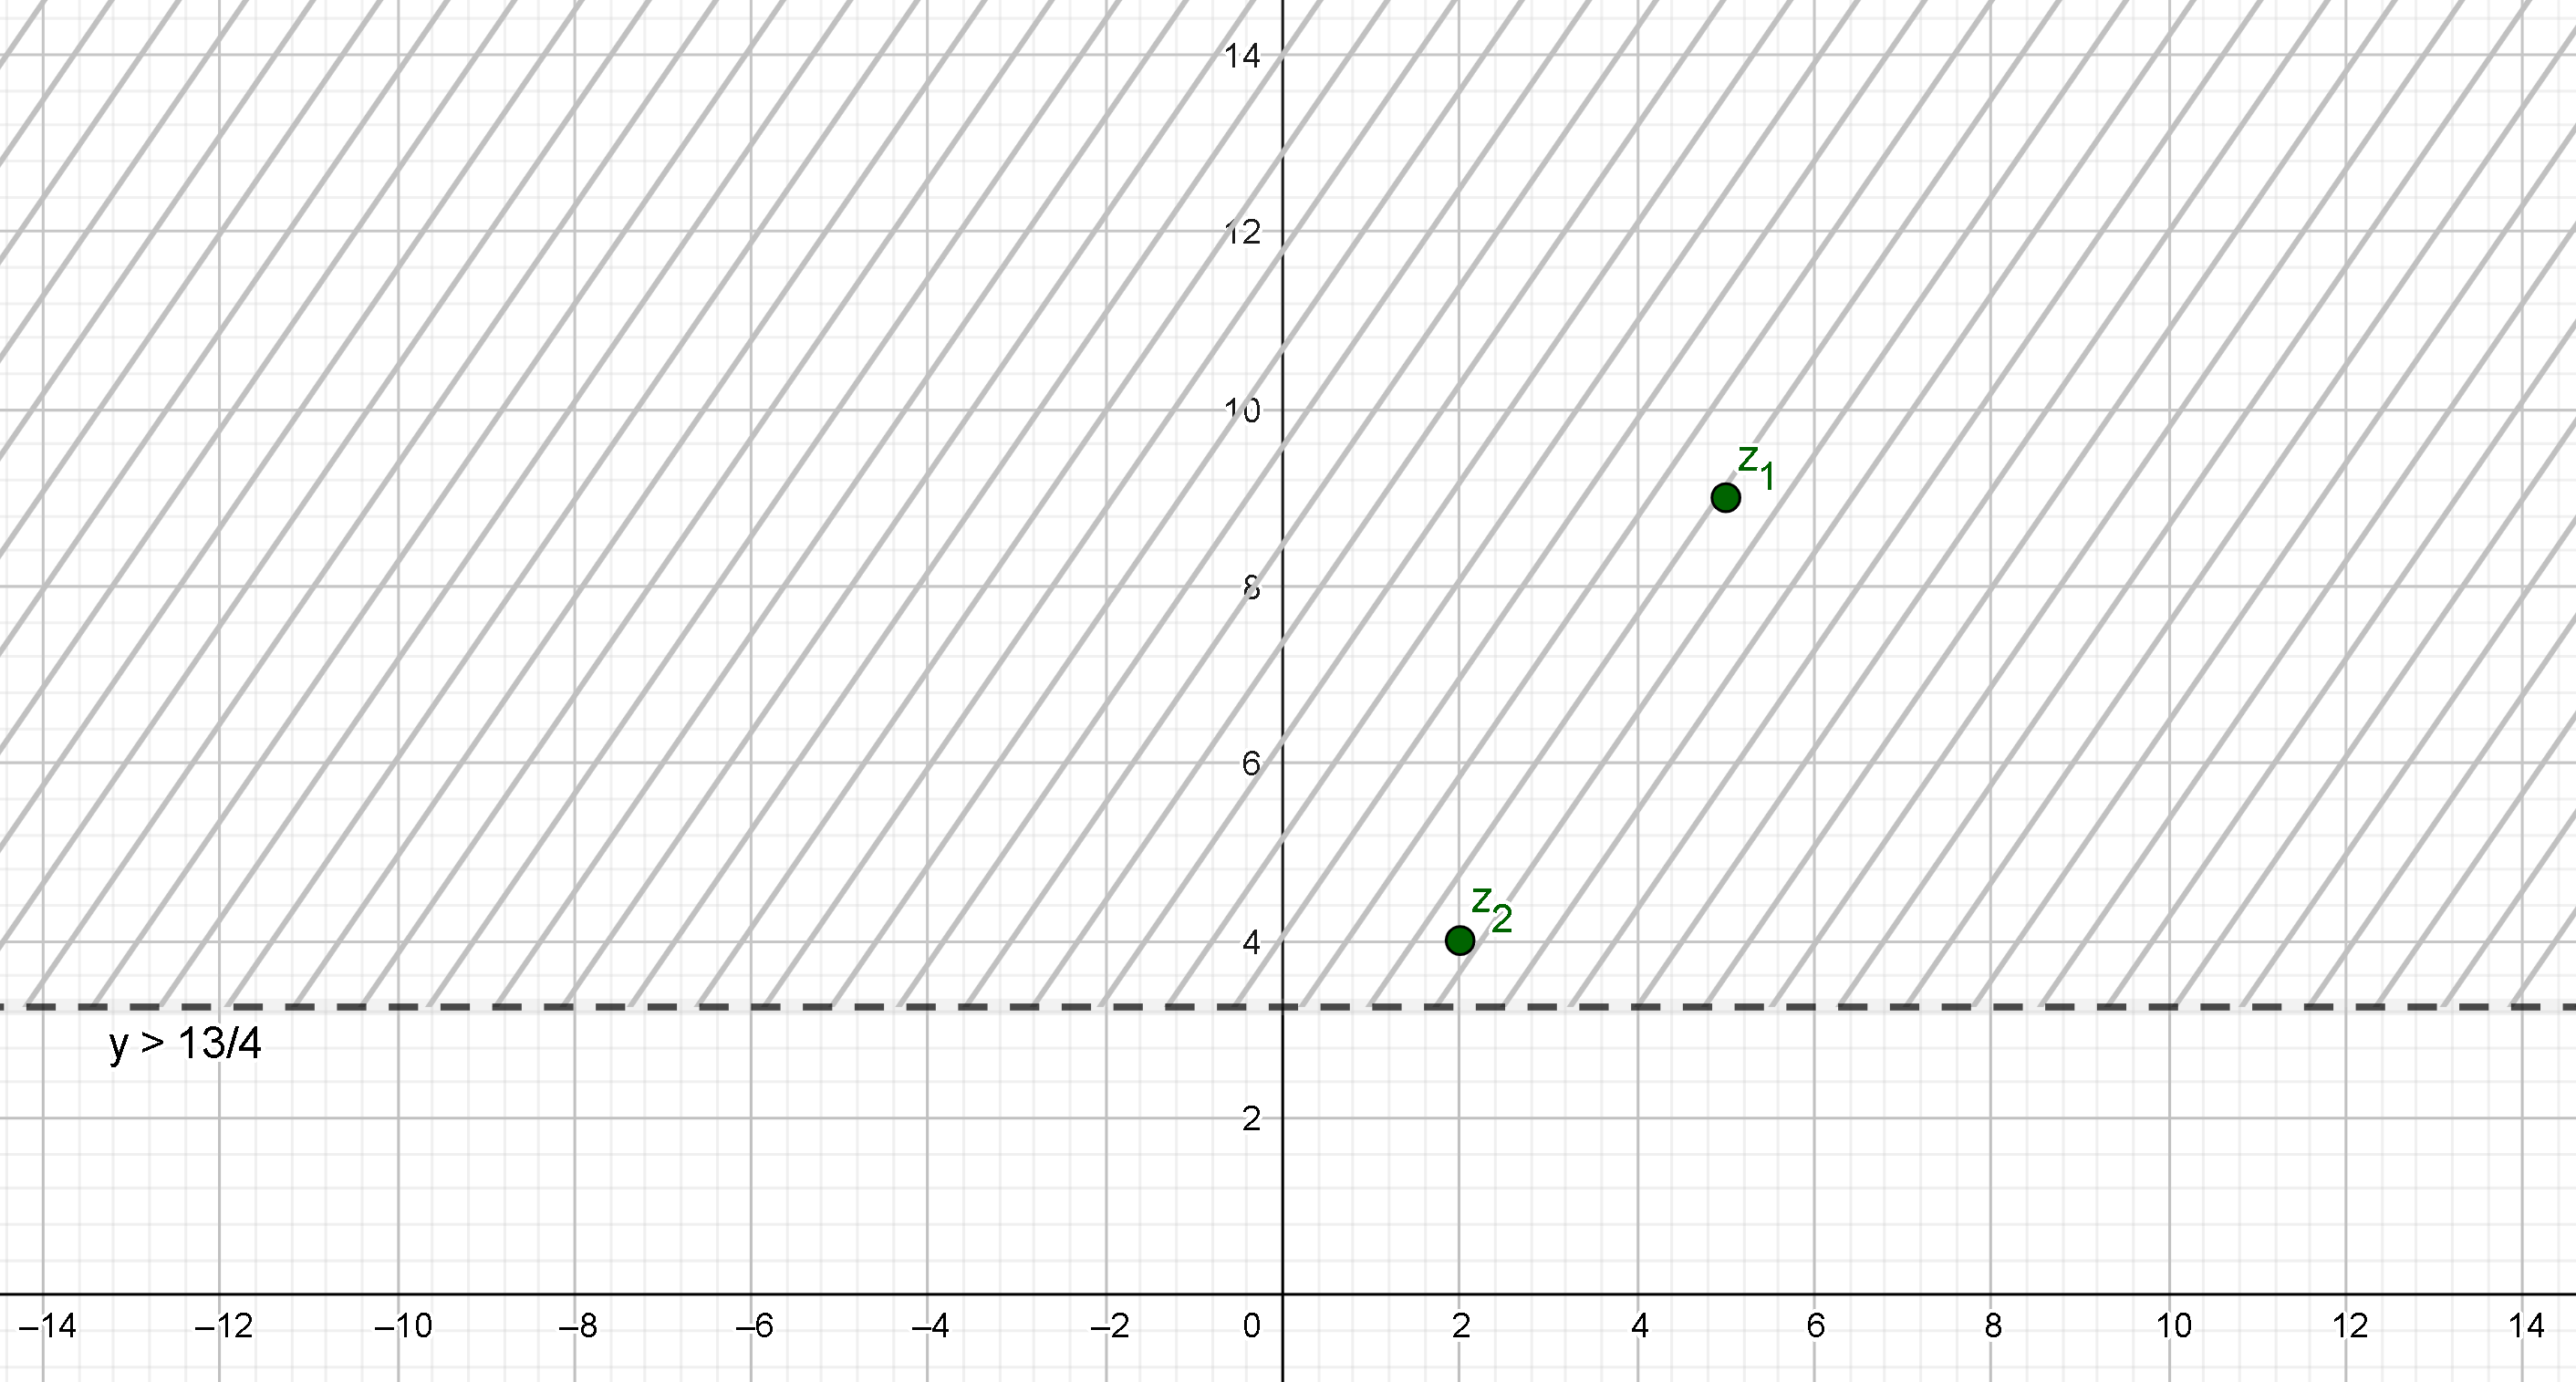
\includegraphics[width=15cm]{Gra-Ej-11.png}
\end{center}

\textcolor{ao(english)}{\ding{47}} Comprobación de puntos $y\,>\,\dfrac{13}{4}$:

$$\mathnormal{Im}\,(5\,+\,9\,i)\,>\,\dfrac{13}{4} \quad\iff\quad 9\,>\,\dfrac{13}{4}$$

$$\mathnormal{Im}\,(2\,+\,4\,i)\,>\,\dfrac{13}{4} \quad\iff\quad 4\,>\,\dfrac{12}{4}$$

\textcolor{ao(english)}{(\,12\,)} $\bf{\mathnormal{Re}\,(1\,+\,7\,i\,+\,z)\,>\,\dfrac{2}{3}}$.

\end{document}